% \documentclass[11pt]{elsarticle}
\documentclass{elsarticle}

\usepackage{subfiles}
\usepackage{amsmath,amssymb,amsthm,amsfonts}
\usepackage{enumitem}
\usepackage{kantlipsum,graphicx}
\usepackage{caption,subcaption}
\usepackage{multicol,colortbl,multirow}
\usepackage{pgfplots,booktabs,xfrac,floatrow}
\usepackage{xcolor,cancel,bm,tikz}
\usepackage{hyperref}
\usepackage{mathtools}
\usepackage{placeins}
\usepackage{comment}
\usepackage[normalem]{ulem}
\usepackage{parskip}
\usepackage{graphicx}
\usepackage{adjustbox}
\usepackage{float}
\usepackage{tabularx} % Required for tables that stretch to text width
\usepackage{booktabs} % For prettier tables
\usepackage{ltablex}
\usepackage{pdfpages}
\usepackage{listings}
\usepackage{color}
\usepackage{natbib}
\usepackage{cleveref}
\usepackage{csquotes}
% \usepackage{showkeys}

\hyphenation{Timoshenko}

\keepXColumns

% Set up hyperref
\hypersetup{
  colorlinks=true,
  allcolors=black,
  pdftitle={Your Title Here},
}

% Set up theorem environments
\theoremstyle{plain}
\newtheorem{theorem}{Theorem}[section]
\newtheorem{lemma}[theorem]{Lemma}
\newtheorem{proposition}[theorem]{Proposition}
\newtheorem{corollary}[theorem]{Corollary}

\theoremstyle{definition}
\newtheorem{definition}[theorem]{Definition}
\newtheorem{example}[theorem]{Example}
\newtheorem{exercise}[theorem]{Exercise}

\theoremstyle{remark}
\newtheorem{remark}[theorem]{Remark}

% Set up equation numbering
\numberwithin{equation}{section}

% Define custom commands
\newcommand{\hcancel}[2][black]{%
  \setbox0=\hbox{$#2$}%
  \rlap{\raisebox{.45\ht0}{\textcolor{#1}{\rule{\wd0}{1pt}}}}#2%
}

% Define paired delimiters
\DeclarePairedDelimiter{\abs}{\lvert}{\rvert}
\DeclarePairedDelimiter{\ang}{\langle}{\rangle}

% Define colors
\definecolor{mGreen}{rgb}{0,0.6,0}
\definecolor{mGray}{rgb}{0.5,0.5,0.5}
\definecolor{mPurple}{rgb}{0.58,0,0.82}
\definecolor{backgroundColour}{rgb}{0.95,0.95,0.92}

% Setup the listings package
\lstset{
  language=Matlab,
  basicstyle=\footnotesize\ttfamily,
  backgroundcolor=\color{backgroundColour},
  commentstyle=\color{mGreen},
  keywordstyle=\color{magenta},
  numberstyle=\tiny\color{mGray},
  stringstyle=\color{mPurple},
  breakatwhitespace=false,         
  breaklines=true,                 
  captionpos=b,                    
  keepspaces=true,                 
  numbers=left,                    
  numbersep=5pt,                  
  showspaces=false,                
  showstringspaces=false,
  showtabs=false,                  
  tabsize=2,
  frame=single
}

% \DeclareBibliographyCategory{cited}
% \AtEveryCitekey{\addtocategory{cited}{\thefield{entrykey}}}
\usepackage{geometry}
\geometry{
  left=1.3in,
  right=1.4in,
  top=1.4in,
  bottom=1.4in,
}

\begin{document}

\begin{frontmatter}

\title{Comparison of linear beam theories}

\author{R. du Toit\corref{cor1}}
\ead{u15000258@tuks.co.za}
\cortext[cor1]{Corresponding author}
\author{N.F.J. van Rensburg}
\address{Department of Mathematics, University of Pretoria, Pretoria, South Africa}

\journal{Applied Mathematics and Computation}

\begin{abstract}
Beams, while commonly used in engineering, are complex three-dimensional objects. Simplified models are often used in vibration problems due to their reduced complexity and computational demand. However, the accuracy of these models in practical applications is not always certain. This article extends previous research to examine a two-dimensional cantilever beam model's validity using modal analysis and the Finite Element Method (FEM), comparing its solutions with those of a three-dimensional model. Our findings reveal that the beam's shape is a crucial factor in the model's validity for practical applications. For the appropriate beam shapes, the two-dimensional model is a valid approximation of the three-dimensional model. 
\end{abstract}

\begin{keyword}
	Beam \sep Cantilever Beam \sep Two-Dimensional Model \sep Three-Dimensional Model \sep Vibration Analysis \sep Modal Analysis \sep Finite Element Method
\end{keyword}

\end{frontmatter}

\section{Introduction}
In the article \cite{LVV09}, the authors investigate the validity of a cantilever Timoshenko beam model. Validity refers to how well the solution of the simplified model compare to a more complex higher dimensional model. The reference model in \cite{LVV09} is a two-dimensional cantilever beam model.

In this article, we build upon \cite{LVV09} by further examining the validity of a two-dimensional model for a cantilever beam, using a three-dimensional model as the reference. We follow the same methodology as \cite{LVV09}, employing modal analysis and the Finite Element Method (FEM) to compare the two models. This extention is motivated by the authors of \cite{LVV09}.

To start, the models are presented in a dimensionless variational form. We explain how the two-dimensional model is derived from the three-dimensional model as a special case of plane stress. The well-posedness of the two models is not proved in this article, but the necessary existence and uniqueness results from \cite{VV02} are mentioned.

Next we introduce the concept of modal analysis with a general vibration problem. Through modal analysis, we derive a formal series solution for the vibration issue, which is a linear combination of the problem's eigenvectors and eigenvalues. This approach allows us to compare the solutions of the two models by focusing on a comparison of their eigenvectors and eigenvalues.

We then apply the Finite Element Method (FEM) to the two models and obtain a formula for the models to numerically solve the eigenvalue problem. The article \cite{BV13} provides essential convergence results for the FEM in vibration problems. The textbook \cite{SF73} also offers insights into the convergence of eigenvalues and eigenfunctions in a vibration problem when using FEM. 

Following \cite{LVV09}, by considering the mode shapes, we can match up the eigenvalues and compare them. In the comparison, we consider different shapes of beams that are useful in practical applications. We find that the shape of the beam significantly influences the validity of the two-dimensional model. The results of the comparison are presented in the form of tables and graphs.

The layout of the paper is as follows:
\begin{itemize}
\item Section \ref{sec:LinearMathematicalModels} introduces the linear mathematical models for the three-dimensional, two-dimensional, and Timoshenko beam models.
\item Section \ref{sec:ModalAnalysis} covers modal analysis, compares linear models, and touches on the models' well-posedness.
\item Section \ref{ssec:2D_Model:FEM} outlines the variational problem for the two-dimensional model and applies the Finite Element Method to derive an eigenvalue problem.
\item Section \ref{ssec:3D_Model:FEM} outlines the variational problem for the three-dimensional model and applies the Finite Element Method to derive an eigenvalue problem.
\item Section \ref{sec:validity-of-a-cantilever-timoshenko-beam} examines the validity of the Timoshenko model for a cantilever beam, drawing on results from \cite{LVV09}.
\item Section \ref{sec:validity-of-a-2d-beam} expands on \cite{LVV09} to assess the validity of a two-dimensional model for a cantilever beam.
\item Section \ref{sec:conclusion} concludes the paper.
\end{itemize}



\section{Linear mathematical models} \label{sec:LinearMathematicalModels}
	\subsection{Three-dimensional theory}
		Consider a vector valued displacement function $u$ defined on $\Omega \subset R^3$.

		\subsubsection*{Equation of motion}\label{ssec:3D_Model:EquationOfMotion}
		\begin{eqnarray}
			\rho\partial_t^2 u & = & \textrm{div}T + Q. \label{eq:3D_Model:EM}
		\end{eqnarray} \label{sym:rho} \label{sym:partial_diff} \label{sym:T} \label{sym:Q}

		Here $\rho$ is the density, $T$ is the stress tensor, and $Q$ is the external 
		force per unit volume and $\textrm{div}T$ is the divergence of the tensor $T$ and represented by
		\begin{eqnarray}
			\textrm{div}  T & = &
			\begin{bmatrix}
				\partial_1 \sigma_{11} + \partial_2 \sigma_{12} + \partial_3 \sigma_{13} \\
				\partial_1 \sigma_{21} + \partial_2 \sigma_{22} + \partial_3 \sigma_{23} \\
				\partial_1 \sigma_{31} + \partial_2 \sigma_{32} + \partial_3 \sigma_{33}
			\end{bmatrix}. \label{eq:3D_Model:divT}
		\end{eqnarray}

		Assuming only small vibrations, the stress tensor $T$ is symmetric due to small
		local displacements and rotations. The trace of the stress tensor $T$ is denoted
		\begin{eqnarray}
			\textrm{Tr}(T) & = & \sigma_{11} + \sigma_{22} + \sigma_{23}. \label{eq:stress_tensor_t}
		\end{eqnarray}

		\subsubsection*{Constitutive Equation}
			For an isotropic material, Hooke's law can be written in terms of Young's modulus $E$ and Poisson's ratio $\nu$. And if the principal stresses $\sigma_i$ are all non-zero, then Hooke's law can be written in the following form:
			\begin{eqnarray}
				T = \left( \frac{E}{1+\nu} \right)\mathcal{E} + \frac{\nu E}{(1+\nu)(1-2\nu)}\textrm{Tr}(\mathcal{E})I \label{eq:3D_Model:CE}.
			\end{eqnarray} Here $\mathcal{E}$ is the strain tensor and $T$ is the stress tensor.

			In this form, Hooke's law is the constitutive equation for the three-dimensional model.

			Let $\ell$ represent a significant dimension (e.g., length) of an elastic body and $G$ the shear modulus. Define dimensionless variables and normalized functions as
			\[\tau = \frac{t}{t_0},\ \xi_i = \frac{x_i}{\ell},\ u^*(\xi,\tau) = \frac{u(x,t)}{\ell},\ Q^{*} = \ell G \kappa^2 Q,\ \sigma_{ij}^*(\xi,\tau) = \frac{\sigma_{ij}(x,t)}{G\kappa^2},\]
			where $\kappa^2$ is a dimensionless constant and $\displaystyle t_0 = \ell\sqrt{\frac{\rho}{G\kappa^2}}$. Let $\displaystyle \gamma= \frac{G\kappa^2}{E}$.

			Substituting these into the equation of motion \eqref{eq:3D_Model:EM} gives
			\[\partial_{\tau} u^{*} = \text{div}T^* + Q^*,\]
			where $\displaystyle T^* = \sigma_{i,j}^*(\xi,\tau)$. The dimensionless forms for \eqref{eq:3D_Model:HL} and \eqref{eq:3D_Model:CE} are
			\[\mathcal{E} = \gamma(1+\nu)T^* - \gamma\nu \text{Tr}(T^*)I,\]
			\[T^* = \frac{\mathcal{E}}{\gamma(1+\nu)} + \frac{\nu\text{Tr}(\mathcal{E})I}{\gamma(1+\nu)(1-2\nu)}.\]

			The choice of dimensionless constants follow \cite{LVV09} and allows for a comparison between this model and the Timoshenko beam model.


		\textbf{Equations of motion in dimensionless form}
			\begin{eqnarray}
				\partial_t^2 u & = & \textrm{div}T + Q \label{eq:3D_Model:EM-D}
			\end{eqnarray}
			with
			\begin{eqnarray}
				\textrm{div}  T & = &
				\begin{bmatrix}
					\partial_1 \sigma_{11} + \partial_2 \sigma_{12} + \partial_3 \sigma_{13} \\
					\partial_1 \sigma_{21} + \partial_2 \sigma_{22} + \partial_3 \sigma_{23} \\
					\partial_1 \sigma_{31} + \partial_2 \sigma_{32} + \partial_3 \sigma_{33}
				\end{bmatrix}.\label{eq:3D_Model:divT-D}
			\end{eqnarray}

		\textbf{Constitutive equations in dimensionless form}
			\begin{eqnarray}
				T = \frac{1}{\gamma(1+\nu)} \mathcal{E} + \frac{\nu}{\gamma(1+\nu)(1-2\nu)}\textrm{Tr}(\mathcal{E})I \label{eq:3D_Model:CE-D}
			\end{eqnarray}

		\subsubsection*{Cantilever model}
			Find a vector valued function $u$, satisfying equations
			\eqref{eq:3D_Model:EM-D} to \eqref{eq:3D_Model:CE-D} and the boundary
			conditions $\displaystyle u = 0$ on part of the boundary and $\displaystyle Tn = 0$ on the rest of the boundary. This will be referred to as \textbf{Problem 3D}.
			
	\subsection{Two-dimensional theory}
		\subsubsection*{General plane stress}
			Stresses acting parallel to a single plane are referred to as plane stress. 
			Consider the right-hand orthonormal set $\left\{e_1, e_2, e_3\right\}$. Without
			loss of generality, assume the stresses act parallel to the $e_1$-$e_2$ plane
			i.e. $\sigma_{3i} = 0$ for all $i$. From Hooke's Law \eqref{DM_H_E} the
			following equations are obtained: \label{sym:e_i}

			\begin{equation}
				\begin{aligned}
					\varepsilon_{11} & =  \gamma  ( \sigma_{11} - \nu \sigma_{22}) \qquad \qquad \varepsilon_{33} & = & - \gamma \nu (\sigma_{11} + \sigma_{22})          \\
					\varepsilon_{22} & =   \gamma (\sigma_{22} - \nu\sigma_{11}) \qquad \qquad \varepsilon_{12}   & = & \  \gamma (1+\nu) \sigma_{12} \label{strain_comp}
				\end{aligned}
			\end{equation}

			and a sufficient condition
			\begin{eqnarray}
				\varepsilon_{13} =  \varepsilon_{23} = 0.
			\end{eqnarray}

			After some manipulation, the following stress-strain relations are obtained:
			components given in \cite{Fung65}.

			\begin{minipage}{.5\linewidth}
				\begin{eqnarray*}
					\sigma_{11} & = & \frac{1}{\gamma(1-\nu^2)} ( \varepsilon_{11} + \nu\varepsilon_{22})\\
					\sigma_{22} & = & \frac{1}{\gamma(1-\nu^2)} (\nu \varepsilon_{11} + \varepsilon_{22}).
				\end{eqnarray*}
			\end{minipage}%
			\begin{minipage}{.5\linewidth}
				\begin{eqnarray}
					\sigma_{12} & = & \frac{1}{\gamma(1+\nu)} \varepsilon_{12} \label{stress_comp}
				\end{eqnarray}
			\end{minipage}

			Another necessary strain condition for plane stress is found by substituting
			$\sigma_{11}$ and $\sigma_{22}$ from \eqref{stress_comp} into
			$\varepsilon_{33}$ in \eqref{strain_comp} to obtain
			\begin{eqnarray}
				\varepsilon_{33} = -\frac{\nu}{1-\nu} (\varepsilon_{11} + \varepsilon_{22}).\label{plane_stress_neseccary_condition}
			\end{eqnarray}

			This is known as general plane stress. The two-dimensional model is a special case of plane stress.

		\subsubsection*{The two dimensional model}
			Assume that $\sigma_{3i} = 0$ for $i = 1, 2, 3$; $\partial_3 u_1 = 0$, $\partial_3 u_2 = 0$ ($u_1$ and $u_2$ are functions of $x_1$ and $x_2$), and the strain component $\varepsilon_{33} = 0$. Then using the definition of strain 
			\begin{eqnarray}
				\partial_i u_3 = 0 \quad \textrm{ for } i = 1,2,3 \textrm{ on } \Omega.
			\end{eqnarray}

			It follows that $u_3$ is a constant on $\Omega$ and $u$ is a vector valued function in 
			$R^2$ with two-dimensional stress and strain. The out of plane conditions for strain 
			\eqref{plane_stress_neseccary_condition} falls away and Hooke’s law can be written in a 
			two-dimensional form using the stress components as 
			\[ T = \frac{1}{\gamma(1+\nu)}\mathcal{E} + \frac{\nu}{\gamma(1-\nu^2)}\textrm{tr}(\mathcal{E})I.\]

			The equations of motion and constitutive equations follow:
			\subsubsection*{Equation of motion}\label{sssec:2D_Model:EquationOfMotion}
			\begin{eqnarray}
				\partial_t^2 u & = & \textrm{div}T + Q, \label{eq:2D_Model:EM}
			\end{eqnarray}
			where
			\begin{eqnarray}
				\textrm{div} T & = &
				\begin{bmatrix}
					\partial_1 \sigma_{11} + \partial_2 \sigma_{12} \\
					\partial_1 \sigma_{21} + \partial_2 \sigma_{22}
				\end{bmatrix}. \label{eq:2D_Model:DivT}
			\end{eqnarray}
			\subsubsection*{Constitutive equation}\label{sssec:2D_Model:ConstitutiveEquation}
			\begin{eqnarray}
				T = \frac{1}{\gamma(1+\nu)}\mathcal{E} + \frac{\nu}{\gamma(1-\nu^2)}\textrm{Tr}(\mathcal{E}) I. \label{eq:2D_Model:CE}
			\end{eqnarray}

		\subsubsection*{Cantilever model}

			Find a vector valued function $u$, satisfying equations \eqref{eq:2D_Model:EM} to \eqref{eq:2D_Model:CE} and the boundary conditions $u = 0$ on part of the boundary and $Tn = 0$ on the rest of the boundary. This will be referred to as \textbf{Problem 2D}.


	\subsection{Timoshenko theory}
		Consider a Timoshenko beam with no damping defined on the interval $[0,\ell]$.
		Let $w$ represent the transverse displacement and $\phi$ a rotation of the cross-sections of the beam.

		\subsubsection*{Equations of motion}\label{sssec:1D_Model:EquationOfMotion}
			\begin{eqnarray}
				\rho A \partial_t^2 w &=& \partial_x V + Q, \label{eq:1D_Model:EquationOfMotion1}\\
				\rho I\partial_t^2 \phi  &=& V + \partial_x M. \label{eq:1D_Model:EquationOfMotion2}
			\end{eqnarray}\label{sym:A}\label{sym:V}\label{sym:Iinertia}\label{sym:M}\label{sym:phiT}
			In~\eqref{eq:1D_Model:EquationOfMotion1} and \eqref{eq:1D_Model:EquationOfMotion2} $\rho$ denotes the density, $A$ is the area of a cross section, $I$ is the area moment of inertia, $M$ is the moment, $V$ is the shear force and $Q$ is an external force acting on the beam.

		\subsubsection*{Constitutive equations}\label{sssec:1D_Model:ConstitutiveEquation}
			\begin{eqnarray}
				M &=& EI\partial_x \phi, \label{eq:1D_Model:ConstitutiveEquations1}\\
				V &=& AG\kappa^2(\partial_x w - \phi), \label{eq:1D_Model:ConstitutiveEquations2}\label{sym:kappa2T}
			\end{eqnarray}
			$E$ is Young's modulus, $G$ the shear modulus and $\kappa^2$ the shear correction factor.

		\subsubsection*{Dimensionless form}\label{sssec:1D_Model:DimensionlessForm}
			As mentioned in the dimensionless form of the three-dimensional model, the same dimensionless scaling can be applied to the Timoshenko beam theory.

			Set \[\tau = \frac{t}{t_0},\ \xi = \frac{x}{\ell},\ w^*(\xi,\tau) = \frac{w(x,t)}{\ell},\ \phi^*(\xi, \tau) = \phi(x,t).\]

			Dimensionless shear force, moment, and external force density are \[V^{*} = \frac{V}{AG\kappa^2},\ M^{*} = \frac{M}{A G\kappa^2 \ell},\ Q^* = \frac{Q\ell}{A G\kappa^2}.\]

			Use $\displaystyle t_0 = \ell\sqrt{\frac{\rho}{G\kappa^2}}$ as before.

			Using the dimensionless constants from \cite{LVV09}, 
			\[\alpha = \frac{A \ell^2}{I},\ \beta =\frac{AG\kappa^2 \ell^2}{EI},\]
			with \[\frac{\beta}{\alpha} = \gamma,\] where $\gamma$ is the dimensionless parameter from the three-dimensional model.

		\subsubsection*{Dimensionless equations of motion}\label{sssec:1D_Model:DimensionlessEquationsOfMotion}
			\begin{eqnarray}
				\partial_{t}^{2} w &=& \partial_{x}V + Q, \label{eq:1D_Model:EquationOfMotion1D}\\
				\frac{1}{\alpha} \partial_{t}^{2} \phi &=& V + \partial_{x}M.\label{eq:1D_Model:EquationOfMotion2D}
			\end{eqnarray}
		\subsubsection*{Dimensionless constitutive equations}\label{sssec:1D_Model:DimensionlessConstitutiveEquations}
			\begin{eqnarray}
				M &=& \frac{1}{\beta}\partial_x \phi, \label{eq:1D_Model:ConstitutiveEquations1D}\\
				V &=& \partial_x w-\phi. \label{eq:1D_Model:ConstitutiveEquations2D}
			\end{eqnarray}
		The original notation is retained for convenience.

		\textbf{Models and variational forms}
			\subsubsection*{Bilinear forms and integral}
				For $f,g \in T[0,1]$, define the bilinear forms
				\begin{eqnarray}
					c(f,g) & = & \int_0^1  \partial_t^2 f_1 g_1 + \frac{1}{\alpha}\int_0^1  \partial_t^2 f_2g_2, \label{eq:1D_Model:Bilinear} \\
					b(f,g) & = &   \int_0^1 (f_1'-f_2)(g_1' - g_2) + \frac{1}{\beta}\int_0^1 f_2' g_2', \label{eq:1D_Model:Bilinear_c}
				\end{eqnarray}
				Define the integral
				\begin{eqnarray}
				(f,g)
					&=& \int_{0}^1 fg \label{eq:1D_Model:Bilinear_int}
				\end{eqnarray} for all $f,g \in L^2(0,1).$

				\textbf{Remark}
				$L^2(a,b)$ is the space of all square integrable functions on the interval $(a,b)$. The inner product is defined by $\displaystyle (f,g) = \int_a^b fg$, and the induced norm $\displaystyle ||f|| = \int_a^b f^2$.\\

			\subsection*{Pinned-pinned beam}
				Find functions $w$ and $\phi$ satisfying equations \eqref{eq:1D_Model:EquationOfMotion1D} to \eqref{eq:1D_Model:ConstitutiveEquations2D} and the boundary conditions:

				{Boundary Conditions}
				\begin{eqnarray*}
					w(0,\cdot) = 0, \ \ &M(0,\cdot) = 0, \label{eq:1D_Model:ProblemT1BC1}\\
					w(1,\cdot) = 0, \ \ &M(1,\cdot) = 0. \label{eq:1D_Model:ProblemT1BC2}
				\end{eqnarray*}

				This will be referred to as \textbf{Problem T-1}. Define the set of test functions $T[0,1]$ for Problem T-1 as
				\begin{eqnarray*}
					T[0,1] &:=&  \left\{f \in C^1[0,1] \ | \ f(0) = f(1) = 0 \right\} \times C^1[0,1]
				\end{eqnarray*}

				Then the variational problem for Problem T-1 is given by
				\subsubsection*{Problem T-1V}\label{sssec:1D_Model:ProblemT1V}
					Find a function ${u} = \langle w, \phi \rangle$ such that for all $t >0$, ${u} \in  T[0,1]$ satisfying
					\begin{eqnarray}
						c(\partial_t^2 u,{\phi}) &=& -b({u},{\phi}) + (Q,{\phi})
					\end{eqnarray} for each ${\phi} = \langle v, \psi \rangle \in T[0,1]$.

			\subsection*{Cantilever beam}
				Find functions $w$ and $\phi$ satisfying equations \eqref{eq:1D_Model:EquationOfMotion1D} to \eqref{eq:1D_Model:ConstitutiveEquations2D} and the boundary conditions:

				{Boundary Conditions}
				\begin{eqnarray*}
					w(0,\cdot) = 0, \ \ &\phi(0,\cdot) = 0, \label{eq:1D_Model:ProblemT2BC1}\\
					M(1,\cdot) = 0, \ \ &V(1,\cdot) = 0. \label{eq:1D_Model:ProblemT2BC2}
				\end{eqnarray*}

				This will be referred to as \textbf{Problem T-2}.  Define the set of test functions $T[0,1]$ for Problem T-2 as
				\begin{eqnarray*}
					T[0,1] &:=& \left\{g \in C^1[0,1] \ | \ g(0) = 0 \right\} \times \left\{g \in C^1[0,1] \ | \ g(0) = 0 \right\}
				\end{eqnarray*}

				Then the variational problem for Problem T-2 is given by
				\subsubsection*{Problem T-2V}\label{sssec:1D_Model:ProblemT1V}
					Find a function ${u} = \langle w, \phi \rangle$ such that for all $t >0$, ${u} \in  T[0,1]$ satisfying
					\begin{eqnarray}
						c(u,{\phi}) &=& -b({u},{\phi}) + (Q,{\phi}) \label{var_form_timo}
					\end{eqnarray} for each ${\phi} = \langle v, \psi \rangle \in T[0,1]$. 	
				
\section{Modal analysis and comparison of linear models}\label{sec:ModalAnalysis}	

	\subsection*{Existance and uniqueness of solutions}
		Our two models, the three-dimensional modela and the two-dimensional model, concern the vibration of elastic bodies. These type of models have a similar variational form as the wave equation and are called second order hyperbolic type problems. The articles \cite{VV02} and \cite{VS18} provide existence and uniqueness results for these type of problems. In \cite{VV02}, it is assumed that $b$ is symmetric. \cite{VS18} extends the results of \cite{VV02} to the case where $b$ is not symmetric. For the models in the article, \cite{VV02} is a sufficient reference.

		Let $V$, $W$ and $X$ be Hilbert spaces such that $V \subset W \subset X$.
		\begin{itemize}
			\item[] X is the global space with inner product $(\cdot,\cdot)_X$ and the induced norm $||\cdot||_X$.
			\item[] W is the inertia space with inner product $(\cdot,\cdot)_W$ and the induced norm $||\cdot||_W$.
			\item[] V is the energy space with inner product $(\cdot,\cdot)_V$ and the induced norm $||\cdot||_V$.
		\end{itemize}

		Consider a general second order hyperbolic type problem GVar. This general problem is used by the 
		authors of \cite{VV02} to prove existence and uniqueness results. The models in this article are 
		special cases of this general problem.

		\subsubsection*{Problem GVar}\label{sssec:existence:ProblemGVar}
		Given a function $f:J\rightarrow X$, find a function $u\in C(J,\ X)$ such that $u'$ is continuous at $0$ with respect to $\Vert \cdot \Vert_{W}$ and for each $t\in J,\ u(t)\in V,\ u'(t) \in V,\ u''(t)\in W$ and
		\begin{eqnarray}
			c(u''(t),v)+a(u'(t),v)+b(u(t),v)= (f(t),v)_{X} \ \ \ \ \textrm{for each} \ v \in V, \label{eq:existence:ProblemGVar}
		\end{eqnarray}
		while $u(0)=u_{0},\ \ \ u'(0)=u_{1}$.


		The following assumptions are made in \cite{VV02} for the existence results.
		\begin{itemize}
			\item[] \textbf{A1} - $V$ is dense in $W$ and $W$ is dense in $X$.

			\item[] \textbf{A2} - There exists a positive constant $C_{W}$ such that $\Vert w\Vert_{X} \leq C_{W}\Vert w\Vert_{W}$ for each $ w\in W$.

			\item[] \textbf{A3} - There exists a positive constant $C_{V}$ such that $\Vert v\Vert_{W} \leq C_{V}\Vert v\Vert_{V}$ for each $v \in V$.

			\item[] \textbf{A4} - The bilinear form $a$ is non-negative, symmetric and bounded on $V$, i.e. there exists a positive constant $K_a$ such that for $\displaystyle u,v \in V$, \[|a(u,v)| \leq K_a\Vert u \Vert_V \Vert v \Vert_V.\]
		\end{itemize}

		Proving that these assumptions are satisfied for the models in this article too much work to include in this article. The existence and uniqueness results of \cite{VV02} are used in this article without proof.

	\subsection*{Modal Analysis}
		Modal analysis is a important concept in the study of vibration of elastic bodies and also useful in the comparison of linear models. The following section is a short discussion of the basic concepts of modal analysis and how it enables the comparison of linear models.

		The discussion follows the article \cite{CVV18}, excluding damping. Consider Problem GVar with no damping or external forces.

		\subsubsection*{Problem GVar}\label{sssec:existence:ProblemGVar}
		Find a function $u \in C(J,\ X)$ such that $u'$ is continuous at $0$ with respect to $\Vert \cdot \Vert_{W}$, and for each $t \in J$, $u(t) \in V$, $u'(t) \in V$, $u''(t) \in W$, satisfying
		\begin{eqnarray}
		c(u''(t),v)+b(u(t),v) = 0 \ \ \ \ \textrm{for each} \ v \in V, \label{eq:existence:ProblemGVarHom}
		\end{eqnarray}
		with initial conditions $u(0) = u_0$ and $u'(0) = u_1$.

		Now consider a trial solution $u(t) = T(t)x$ with $x \in V$ and $x \neq 0$. Substituting this trial solution into \eqref{eq:existence:ProblemGVarHom} results in
		\begin{eqnarray*}
			b(T(t)x,v) = - c(T''(t)x,v).  \label{eq:existence:ProblemGVarHom:Substitution}
		\end{eqnarray*}

		Due to the linearity of the bilinear form, this equation can be rewritten as
		\begin{eqnarray*}
			T(t)b(x,v) = - T''(t)c(x,v).
		\end{eqnarray*}

		Dividing both sides by $T(t)$ gives
		\begin{eqnarray*}
			b(x,v) = - \frac{T''(t)}{T(t)}c(x,v).
		\end{eqnarray*}

		Therefore $\displaystyle -\frac{T''(t)}{T(t)}$ must be constant. Suppose that $\displaystyle \frac{T''(t)}{T(t)} = -\lambda$. The existence of such a $\lambda$ is uncertain at this point. So we consider the following eigenvalue problem.

		Find a real number $\lambda$ and a $x \in V$ with $x \neq 0$ such that
		\begin{eqnarray*}
			b(x,y) = \lambda c(x,y) \ \ \ \ \textrm{ for each } \ y \in V.
		\end{eqnarray*}

		A solution to the eigenvalue problem consists of an eigenvalue $\lambda$ with corresponding eigenvector $x$. 

		The article \cite{CVV18} is a convenient reference to show that the eigenvalue problem has a solution if the following assumption, aditional to \textbf{A1}, \textbf{A2}, \textbf{A3} and \textbf{A4},  is satisfied:

		\begin{itemize}
			\item[] \textbf{A5} - The embedding of $V$ into $W$ is compact.
		\end{itemize}


		Using these assumptions, the authors of \cite{CVV18} prove that there exists a complete orthonormal sequence of eigenvectors for the eigenvalue problem with a corresponding sequence of eigenvalues. These eigenvalues are positive and the orthogonality is with respect to the bilinear form $c$. In fact it is also orthogonal with respect to the bilinear form $b$,
		\begin{eqnarray*}
			b(x_i, x_j) = \lambda_i c(x_i, x_j) = 0, \ \ \ \ \textrm{ for each } \ i \neq j.
		\end{eqnarray*}

		Also the sequence of normalized eigenvectors ${x_i}$ forms an orthonormal basis in $W$ and sequence of eigenvalues ${\lambda_i}$ is an infinite sequence with $\lambda_n \rightarrow \infty$ as $n \rightarrow \infty$. 

		Following these results from \cite{CVV18}, for any $u \in V$, $\displaystyle u = \sum_{i=1}^{\infty} a_i x_i$. These coefficients $a_i$ are generalized Fourier coefficients of $u$ with respect to the eigenvectors $x_i$. Therefore, for any $u \in V$,
		\begin{eqnarray*}
			u = \sum_{i=1}^{\infty} a_i x_i. = \sum_{i=1}^{\infty} c(u, x_i)x_i.
		\end{eqnarray*}

		Now that the eigenvalue problem has many solutions, the following ordinary differentiable equation can be considered,
		\begin{eqnarray*}
			T_n'' + \lambda T_n = 0. 
		\end{eqnarray*}

		Since this differential equation is a simple second order differential equation, $T_n(t)$ has the following possible solutions:
		\begin{flalign}
			T_n(t) &=  A_n \cos(\sqrt{\lambda_n} t) + B_n \sin(\sqrt{\lambda_n} t) \quad \textrm{ if } \lambda_n > 0, \label{lambda_1}
		\end{flalign}

		Then combining the solutions of the eigenvalue problem and the differential equation, the formal series solution for the boundary value problem is
		\begin{eqnarray}
			u(t) = \sum_{n=1}^{\infty} T_n(t)x_n. \label{eq:1D_Model:ModalAnalysisSeriesSolution}
		\end{eqnarray}


	\subsection*{Validity of series solution}
		Consider the following question: When is the formal series solution valid for the vibration problem with initial values $u(0) = u_0$ and $u'(0) = u_1$? To answer this question, we again refer to the article \cite{CVV18}.

		In the article, the validity of the series solution is proved using energy norms, where the energy $\mathcal{E}$ a function $u$ given by \label{sym:Energy}
		\begin{eqnarray}
			\mathcal{E} (t) = \frac{1}{2} b(u(t), u(t)) + \frac{1}{2} c(u'(t), u'(t)). \label{eq:1D_Model:ModalAnalysisEnergy}
		\end{eqnarray}

		Then,
		\begin{eqnarray*}
			\mathcal{E}'(t) & = & b(u(t), u'(t)) + c(u'(t), u''(t)),\\
							& = & 0 \ \ \ \ \ \ \ \textrm{ following from \eqref{eq:existence:ProblemGVarHom}}. 
		\end{eqnarray*}

		Therefore $\mathcal{E}(t) = \mathcal{E}(0)$ for all $t>0$. For the case of weak damping, it can be proved that $\mathcal{E}(t) \leq \mathcal{E}(0)$ for all $t>0$ which is the case of \cite{CVV18}.

		Denote the partial sum $u^{N}(t) = \sum_{n=1}^{N} T_{n}(t)w_n$. Ideally
		\begin{eqnarray*}
			u_0^{N} = \sum_{n=1}^{N} T_n(0) w_n \ \ \textrm{ and } \ \ u_{1}^{N} =\sum_{n=1}^{N} T'_n(0) w_n,
		\end{eqnarray*}
		but $T_n$ is not uniquely defined by the differential equation.

		Substitution shows that these partial sums with initial conditions $u^N(0) = u^N_0$ and $(u^N)'(0) = u^N_1$ are solutions for \eqref{eq:existence:ProblemGVarHom} in Problem GVar.

		The authors then define an error function $u^E_N = u - u^N$. Since both $u$ and $u^N$ satisfies \eqref{eq:existence:ProblemGVarHom}, so does this error function with the following the initial conditions, $u^E_N(0) = u_0 - u^N_0$ and $(u^E_N)'(0) = u_1 - u^N_1$.

		Let $\mathcal{E}$ denote the energy of the error function $u^E_N$. Since $\mathcal{E}(t) = \mathcal{E}(0)$ for all $t>0$ it follows that, 
		\begin{eqnarray}
			||u(t) -  u^N(t)||_V^2 + ||u'(t) - (u^N)'(t)||^2_W = ||u_0 - u^N_0||_V^2 + ||u_1 - u^N_1||_W^2. \label{eq:inequality}
		\end{eqnarray}

		Now, $u_0$ and $u_1$ are given in Problem GVar. Therefore the generalized Fourier coefficients for $u_0$ and $u_1$ must be used to compute $u_0^N$ and $u_1^N$. These Fourier coefficients are $\displaystyle u_0^N = \sum_{n=1}^{N} b(u_0, w_n)w_n$ and $\displaystyle u_1^N = \sum_{n=1}^{N} c(u_1, w_n)w_n$.

		Then $||u_0 - u^N_0||_V^2 \rightarrow 0$ and $||u_1 - u^N_1||_W^2 \rightarrow 0$ as $N \rightarrow \infty$. Therefore $\mathcal{E}(t) \rightarrow 0$ as $N \rightarrow \infty$ by \eqref{eq:inequality}.

		It follows that the partial sums of the series solution converges to the solution $u$ as the initial conditions $u_0^N$ and $u_1^N$ converges to $u_0$ and $u_1$ respectively.

	\subsection*{Comparison of models}
		The results on modal analysis and the validity of the series solution enable the comparison of different linear models. The solution of the model problems can be expressed as a series solution of the eigenvalues and eigenvectors of the models. Therefore the models can be compared by comparing the eigenvalues and eigenvectors of the models.

		The validity of the series solution also ensures that the comparisons remain valid, no matter the inital distrubance of the models. Suppose that for the same initial conditions, $u_b$ and $u_w$ are the exact solutions. A comparison of the exact solutions are not possible, but the partial sums can be compared if the bounds for the errors $u_b - u^N_b$ and $u_w - u^N_w$ can be guaranteed.

\section{Cantilever two-dimensional model in variational form}\label{ssec:2D_Model:FEM}
Let $\{e_1,e_2\}$ be a right-handed orthonormal basis for $R^2$. Denote the elastic body by $\Omega \in R^2$, with $(0,0)$ as the point of reference. For a rectangular cross-section, the body $\Omega$ can be described as,
\begin{eqnarray*}
	\Omega = \left \{ x \in E_2 \ | \ 0 \leq x_1 \leq 1, \ -\frac{h}{2} \leq x_2 \leq \frac{h}{2} \right \},
\end{eqnarray*} 
$\partial \Omega$ denotes the boundary of the body. $\Sigma$ is the part of the boundary where $x_1 = 0$ and here the boundary condition is $u = 0$. $\Gamma$ is the remainder of the boundary where $Tn = 0$.

\FloatBarrier

\begin{figure}[h!]
	\centering
	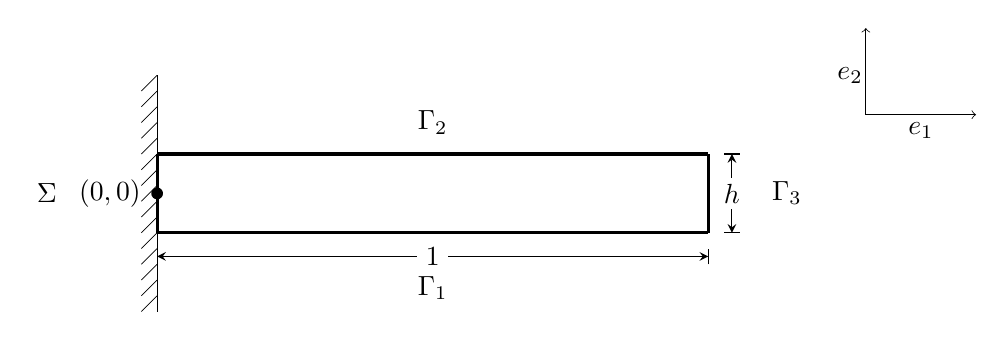
\begin{tikzpicture}
		
		\draw[line width = 0.4mm] (0,0.5) -- (7,0.5);
		\draw[line width = 0.4mm] (0,-0.5) -- (7,-0.5);
		\draw[line width = 0.4mm] (7,-0.5) -- (7,0.5);
		\draw[line width = 0.4mm] (0,-0.5) -- (0,0.5);
		
		\draw[line width = 0.1mm] (0,1.5) -- (0,-1.5);
		
		\draw[line width = 0.1mm] (0,1.5) -- (-0.2,1.3);
		\draw[line width = 0.1mm] (0,1.3) -- (-0.2,1.1);
		\draw[line width = 0.1mm] (0,1.1) -- (-0.2,0.9);
		\draw[line width = 0.1mm] (0,0.9) -- (-0.2,0.7);
		\draw[line width = 0.1mm] (0,0.7) -- (-0.2,0.5);
		\draw[line width = 0.1mm] (0,0.5) -- (-0.2,0.3);
		\draw[line width = 0.1mm] (0,0.3) -- (-0.2,0.1);
		\draw[line width = 0.1mm] (0,0.1) -- (-0.2,-0.1);
		\draw[line width = 0.1mm] (0,-0.1) -- (-0.2,-0.3);
		\draw[line width = 0.1mm] (0,-0.3) -- (-0.2,-0.5);
		\draw[line width = 0.1mm] (0,-0.5) -- (-0.2,-0.7);
		\draw[line width = 0.1mm] (0,-0.7) -- (-0.2,-0.9);
		\draw[line width = 0.1mm] (0,-0.9) -- (-0.2,-1.1);
		\draw[line width = 0.1mm] (0,-1.1) -- (-0.2,-1.3);
		\draw[line width = 0.1mm] (0,-1.3) -- (-0.2,-1.5);
		
		\node at (7.3,0) {$h$};
		\draw[-stealth] (7.3,0.2) -- (7.3,0.5);
		\draw (7.2,0.5) -- (7.4,0.5);
		\draw[-stealth] (7.3,-0.2) -- (7.3,-0.5);
		\draw (7.2,-0.5) -- (7.4,-0.5);
		
		\node at (3.5,-0.8) {$1$};
		\draw[stealth-] (0,-0.8) -- (3.3,-0.8);
		\draw[stealth-] (7,-0.8) -- (3.7,-0.8);
		\draw (7,-0.9) -- (7,-0.7);
		
		\draw[line width = 0.1mm,->] (9,1) -- (10.4,1);
		\draw[line width = 0.1mm,->] (9,1) -- (9,2.1);
		\node at (9.7,0.8) {$e_1$};
		\node at (8.8,1.5) {$e_2$};
		
		\node at (-0.6,0) {$(0,0)$};
		\node at (0,0)[circle,fill,inner sep=1.5pt]{};

		% Add Σ at x_1 = 0
		\node at (-1.4,0) {$\Sigma$};
		
		% Add Γ₁ at x_2 = -h/2
		\node at (3.5,-1.2) {$\Gamma_1$};
		
		% Add Γ₂ at x_2 = h/2
		\node at (3.5,0.9) {$\Gamma_2$};
		
		% Add Γ₃ at x_1 = 1
		\node at (8,0) {$\Gamma_3$};
		
	\end{tikzpicture}
\end{figure} 

\FloatBarrier

\subsubsection*{Problem 2DV}\label{sssec:2D_Model:Problem2D1VChp5}
The bilinear forms and integral function is defined by
\begin{eqnarray}
	b(u,\phi) & = & \int_\Omega~c_1\textrm{Tr}({\cal E}\Phi)+ c_2\textrm{Tr}({\cal E})
	\textrm{Tr}(\Phi) ~dA, \label{eq:2D_Model:BilinearChp5}\\
	c(\partial_t^2 u,\phi) & = & \int_\Omega~ (\partial^2_t u) \cdot \phi~dA, \label{eq:2D_Model:Bilinear_cChp5}\\
	(f,g) &=& \int_{\Omega} f\cdot g \ dA, \label{eq:2D_Model:Bilinear_intChp5}
\end{eqnarray}
with $\displaystyle c_1 = \frac{1}{\gamma(1+\nu)}$ and $\displaystyle c_2 = \frac{\nu}{\gamma(1-\nu^2)}$.

Define the test function space 
\begin{eqnarray*}
	T(\Omega) & = & \left\{ \phi \in C^1(\bar{\Omega}) \ | \ \phi = 0 \ \textrm{ on } \ \Gamma \right\}.
\end{eqnarray*}

Find a function $u$ such that for all $t>0$, $u \in T(\Omega)$ and 
\begin{align}
	c(u,\phi) = -b(u,\phi) + (Q,\phi) \label{eq:2D_Model:Problem2D1VEqChp5}
\end{align}
for all $\phi \in T(\Omega)$.


\subsection*{Galerkin approximation}\label{2d_FEM_G}
To apply the Finite Element Method to Problem 2DV, $\Omega$ must be discretized by dividing it into rectangular elements, suitable for its rectangular cross-section. This process involves creating a grid with $n = n_1 \times n_2$ nodes across $\Omega$.

A set of $n$-dimensional linear independent basis functions is defined, particularly for the two-dimensional model, as 
$$B = \{\langle\phi_1, 0\rangle, \langle\phi_2, 0\rangle,...,\langle\phi_{n}, 0 \rangle,\langle 0,\phi_1\rangle,\langle 0 ,\phi_2\rangle,...,\langle 0,\phi_{n}\rangle \}.$$ 
These functions, chosen as piecewise Hermite bi-cubic functions $\phi_i$, offer quicker convergence and the ability to derive solution derivatives, despite their increased complexity compared to bi-linear functions.

The subset of basis functions from $B$ that meet the criteria of the test function space $T(\Omega)$ are termed admissible basis functions, denoted by $\delta_j$, where each $\delta_j$ is a distinct element of $B$. These can be enumerated and presented as the set 
$$A = \{\delta_1, \delta_2,..., \delta_k \}$$ 
for some $k \leq 2n$.

Define the space
\begin{eqnarray*}
S^h & = & \textrm{span}\left(\left\{\delta_i \ | \ i = 1,2,...,k \right\} \right).
\end{eqnarray*}

For each function $u^h \in S^h$, $u^h$ can be expressed as
\begin{eqnarray*}
	u^h = \sum_{i = 1}^{k} u_i(t) \delta_{i}(x).
\end{eqnarray*}

Substitution of $u^h$ into Problem 2DV, results in the following Galerkin Approximation, denoted by Problem 2DG.

\subsubsection*{Problem 2DG}
Find a function $u^h$ such that for all $t>0$, $u^h \in S^h$ and
\begin{eqnarray*}
	(u^h, \phi_i) & = & -b(u^h,\phi_i) + (Q^I, \phi_i)
\end{eqnarray*} for $i = 1,2,...,k$. $Q^I$ is scalar vector obtained after interpolating the function $Q$ over the rectangular grid $\Omega$. i.e. $Q^I_{i,j} = Q(x_i,x_j)$ for $i = 1,2,...,n_1$ and $j = 1,2,...,n_2$.


Consider the following standard Finite Element Method matrices

\noindent\begin{minipage}{.5\linewidth}
	\begin{eqnarray*}
		\mathbf{M}_{j,i} & = & \int_{\Omega} \phi_i \phi_j ~dA \\
		\mathbf{{K}_{11}}_{j,i} & = & \int_{\Omega} \partial_1\phi_i \partial_1\phi_j~dA\\
		\mathbf{{K}_{22}}_{j,i} & = & \int_{\Omega} \partial_2\phi_i \partial_2\phi_j~dA
	\end{eqnarray*}
\end{minipage}%
\begin{minipage}{.5\linewidth}
	\begin{eqnarray*}
		\mathbf{{K}_{12}}_{j,i} & = & \int_{\Omega} \partial_2\phi_i \partial_1\phi_j~dA\\
		\mathbf{{K}_{21}}_{j,i} & = & \int_{\Omega} \partial_1\phi_i \partial_2\phi_j~dA
	\end{eqnarray*}
\end{minipage}
for $i,j = 1,2,...,k$.

And 
\begin{eqnarray*}
	{M_{F}}_{j,i} = \int_{\Omega}  \phi_i \phi_j~dA
\end{eqnarray*}

for $i = 1,2,...,k$ and for $j =1,2,...,2n$.

Define the following matrices:
\begin{eqnarray*}
	K_1 & = & \frac{1}{\gamma(1-\nu^2)} \mathbf{K_{11}} + \frac{1}{2\gamma(1+\nu)}\mathbf{K_{22}} \label{eq:2DFEM:K1} \\
	K_2 & = & \frac{\nu}{\gamma(1-\nu^2)} \mathbf{K_{21}} + \frac{1}{2\gamma(1+\nu)}\mathbf{K_{12}}\label{eq:2DFEM:K2}\\
	K_3 & = & \frac{\nu}{\gamma(1-\nu^2)} \mathbf{K_{12}} + \frac{1}{2\gamma(1+\nu)}\mathbf{K_{21}}\label{eq:2DFEM:K3}\\
	K_4 & = & \frac{1}{\gamma(1-\nu^2)} \mathbf{K_{22}} + \frac{1}{2\gamma(1+\nu)}\mathbf{K_{11}}\label{eq:2DFEM:K4}
\end{eqnarray*}

Using the standard FEM matrices and matrices $K_1$-$K_4$, the following concatenated matrices are defined.
\begin{eqnarray}
	\begin{aligned}
		K = 
		\begin{bmatrix}
			K1 & K2\\
			K3 & K4
		\end{bmatrix}
	\end{aligned}
	\ \ \ \ \ \ \ \ \
	\begin{aligned}
		M_f = 
		\begin{bmatrix}
			M_{F} & O_{F}\\
			O_{F} & M_{F}
		\end{bmatrix}
	\end{aligned}\label{eq:2DFEM:K+M}
\end{eqnarray}

\begin{eqnarray}
	M = 
	\begin{bmatrix}
		\mathbf{M} & O \\
		O & \mathbf{M}
	\end{bmatrix}\label{eq:2DFEM:M}
\end{eqnarray}

The matrices ${O}$ and ${O_f}$ are the zero matrices of the same size as $\mathbf{M}$ and ${M_f}$ respectively.

Using \eqref{eq:2DFEM:K+M} and \eqref{eq:2DFEM:M}, Problem 2DG is rewritten as a system of ordinary differential equations. This system is referred to as Problem 2DODE.

\subsubsection*{Problem 2DODE}
Find a function $\bar{u} \in S^h$ such that
\begin{eqnarray}
	M\ddot{\bar{u}} & = & K\bar{u} + M_{f}Q^I.
\end{eqnarray} With $\bar{u}$ in the form $\bar{u} = \langle u, \partial_1 u, \partial_2 u, \partial_{12} u \rangle$.

\textbf{Remark} This form of $\bar{u}$ is determined by the use of the bi-cubic basis functions.

\subsection*{Eigenvalue problem}\label{2dFEM_EP}
For the eigenvalue problem, assume that there is no external force, $M_{f}Q^I = 0$, so that 
\begin{eqnarray}
		M\ddot{\bar{u}} & = & K\bar{u}.\label{eq:2DFEM:M2}
\end{eqnarray}
It is known that a system of ordinary differential equations has a general solution of the form $e^{rt}$. Suppose that $\bar{w} = e^{\lambda t} \bar{u}$ is a solution for \eqref{eq:2DFEM:M2}. In this solution, $\lambda$ is an eigenvalue and $\bar{u}$ a corresponding eigenfunction. Substitution into \eqref{eq:2DFEM:M2} results in
\begin{eqnarray*}
	M\lambda e^{\lambda t}\bar{u} & = & Ke^{\lambda t}\bar{u}.
\end{eqnarray*}
Since $e^{\lambda t} > 0$ for all values of $\lambda t$, we can cancel it from both sides of the equation and formulate the eigenvalue problem Problem 2DE.

\subsubsection*{Problem 2DE}
Find a real number $\lambda$ and a function $\bar{u} \in S^h$ such that
\begin{eqnarray}
	M\lambda{\bar{u}} & = & K\bar{u}.
\end{eqnarray}

\section{Cantilever three-dimensional model in variational form} \label{ssec:3D_Model:FEM}
	Let $\{e_1,e_2,e_3\}$ be a right-handed orthonormal basis for $R^3$. Denote the elastic body as $\Omega \in R^3$ with $(0,0,0)$ the point of reference. For a rectangular cross-section, the body $\Omega$ can be described as
	\begin{eqnarray*}
		\Omega = \left\{ x \in R^3 \ | \ 0 \leq x_1 \leq 1, \ -\frac{h}{2} \leq x_2 \leq \frac{h}{2} , \ -\frac{b}{2} \leq x_3 \leq \frac{b}{2}\right \}
	\end{eqnarray*}
	$\partial \Omega$ denotes the boundary of the body. $\Sigma$ is the part of the boundary where $x_1 = 0$ and here the boundary condition is $u = 0$. $\Gamma$ is the remainder of the boundary where $Tn = 0$.

	\FloatBarrier
	\begin{figure}[h!]
		\centering
		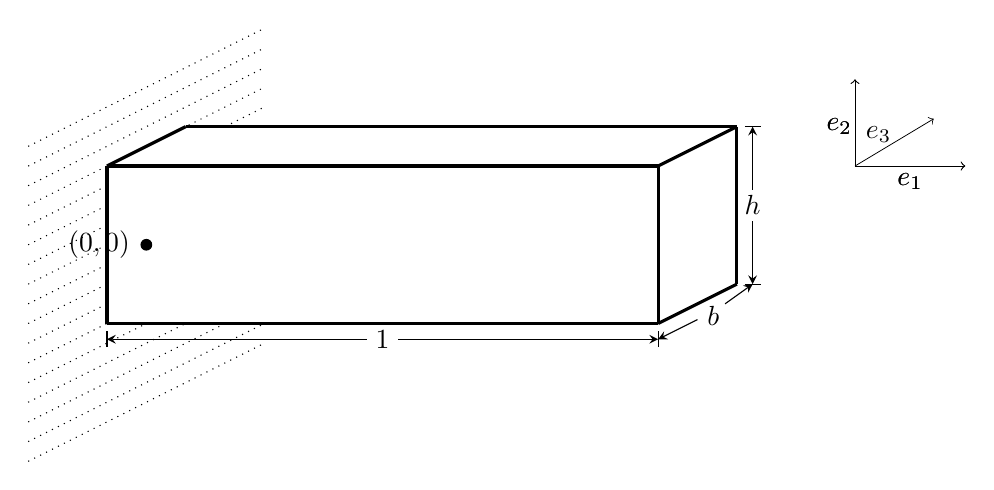
\begin{tikzpicture}
			
			\draw[line width = 0.4mm] (-0.5,1) -- (6.5,1);
			\draw[line width = 0.4mm] (-0.5,-1) -- (6.5,-1);
			\draw[line width = 0.4mm] (6.5,-1) -- (6.5,1);
			\draw[line width = 0.4mm] (-0.5,-1) -- (-0.5,1);
			
			\draw[line width = 0.4mm] (0.5,1.5) -- (7.5,1.5);
			\draw[line width = 0.4mm] (7.5,-0.5) -- (7.5,1.5);
			
			
			\draw[line width = 0.4mm] (-0.5,1) -- (0.5,1.5);
			\draw[line width = 0.4mm] (6.5,1) -- (7.5,1.5);
			\draw[line width = 0.4mm] (6.5,-1) -- (7.5,-0.5);
			
			
			
			\draw[scale=0.5, domain=-3:3, smooth, variable=\x,dotted] plot ({\x}, {0.5*\x+4});
			\draw[scale=0.5, domain=-3:3, smooth, variable=\x,dotted] plot ({\x}, {0.5*\x+3.5});
			\draw[scale=0.5, domain=-3:3, smooth, variable=\x,dotted] plot ({\x}, {0.5*\x+3});
			\draw[scale=0.5, domain=-3:3, smooth, variable=\x,dotted] plot ({\x}, {0.5*\x+2.5});
			
			\draw[scale=0.5, domain=-3:-1, smooth, variable=\x,dotted] plot ({\x}, {0.5*\x+2});
			\draw[scale=0.5, domain=2:3, smooth, variable=\x,dotted] plot ({\x}, {0.5*\x+2});
			
			\draw[scale=0.5, domain=-3:-1, smooth, variable=\x,dotted] plot ({\x}, {0.5*\x+1.5});
			\draw[scale=0.5, domain=-3:-1, smooth, variable=\x,dotted] plot ({\x}, {0.5*\x+1});
			\draw[scale=0.5, domain=-3:-1, smooth, variable=\x,dotted] plot ({\x}, {0.5*\x+0.5});
			\draw[scale=0.5, domain=-3:-1, smooth, variable=\x,dotted] plot ({\x}, {0.5*\x});
			\draw[scale=0.5, domain=-3:-1, smooth, variable=\x,dotted] plot ({\x}, {0.5*\x-0.5});
			\draw[scale=0.5, domain=-3:-1, smooth, variable=\x,dotted] plot ({\x}, {0.5*\x-1});
			\draw[scale=0.5, domain=-3:-1, smooth, variable=\x,dotted] plot ({\x}, {0.5*\x-1.5});
			\draw[scale=0.5, domain=-3:0, smooth, variable=\x,dotted] plot ({\x}, {0.5*\x-2});
			\draw[scale=0.5, domain=-3:1, smooth, variable=\x,dotted] plot ({\x}, {0.5*\x-2.5});
			\draw[scale=0.5, domain=-3:2, smooth, variable=\x,dotted] plot ({\x}, {0.5*\x-3});
			\draw[scale=0.5, domain=-3:3, smooth, variable=\x,dotted] plot ({\x}, {0.5*\x-3.5});
			\draw[scale=0.5, domain=-3:3, smooth, variable=\x,dotted] plot ({\x}, {0.5*\x-4});
			
			%\node at (6.9,1) {$b$};
			%\node at (6.65,0) {$h$};
			%\node at (3.2,-1.2) {$\ell = 1$};
			
			\draw[line width = 0.1mm,->] (9,1) -- (10,1.6);
			\draw[line width = 0.1mm,->] (9,1) -- (10.4,1);
			\draw[line width = 0.1mm,->] (9,1) -- (9,2.1);
			\node at (9.3,1.4) {$e_3$};
			\node at (9.7,0.8) {$e_1$};
			\node at (8.8,1.5) {$e_2$};
			
			\node at (7.7,0.5) {$h$};
			\draw[-stealth] (7.7,0.7) -- (7.7,1.5);
			\draw (7.6,1.5) -- (7.8,1.5);
			\draw[-stealth] (7.7,0.3) -- (7.7,-0.5);
			\draw (7.6,-0.5) -- (7.8,-0.5);
			
			\node at (3,-1.2) {$1$};
			\draw[stealth-] (-0.5,-1.2) -- (2.8,-1.2);
			\draw[stealth-] (6.5,-1.2) -- (3.2,-1.2);
			\draw (6.5,-1.3) -- (6.5,-1.1);
			\draw (-0.5,-1.3) -- (-0.5,-1.1);
			
			\node at (7.2,-0.9) {$b$};
			\draw[stealth-] (7.7,-0.5) -- (7.35,-0.75);
			\draw[stealth-] (6.5,-1.2) -- (7,-0.95);
			
			\draw[line width = 0.1mm,->] (9,1) -- (10.4,1);
			\draw[line width = 0.1mm,->] (9,1) -- (9,2.1);
			\node at (9.7,0.8) {$e_1$};
			\node at (8.8,1.5) {$e_2$};
			
			\node at (-0.6,0) {$(0,0)$};
			\node at (0,0)[circle,fill,inner sep=1.5pt]{};
			
			%\node at (-1.4,-1.3) {$(0,-\frac{h}{2},-\frac{b}{2})$};
			%\node at (-1.4,1) {$(0,\frac{h}{2},-\frac{b}{2})$};
			%\node at (0.5,1.8) {$(0,\frac{h}{2},\frac{b}{2})$};
			
			%\node at (6,-1.3) {$(1,-\frac{h}{2},-\frac{b}{2})$};
			%\node at (6.3,0.7) {$(1,\frac{h}{2},-\frac{b}{2})$};
			%\node at (7.5,1.8) {$(1,\frac{h}{2},\frac{b}{2})$};
			%\node at (8.4,-0.4) {$(1,-\frac{h}{2},\frac{b}{2})$};
			
		\end{tikzpicture}
		
	\end{figure} 

	\FloatBarrier

	\subsubsection*{Problem 3DV}
	The bilinear forms and integral function is defined by
	\begin{eqnarray}
		b(u,\phi) &=& \int_\Omega~c_1\textrm{Tr}({\cal E}\Phi)+ c_2\textrm{Tr}({\cal E})
		\textrm{Tr}(\Phi) ~dV,\\
		c(u,\phi) &=& \int_\Omega~ (\partial^2_t u) \cdot \phi~dV, \\
		(f,g) &=& \int_{\Omega} f\cdot g \ dV, \\
	\end{eqnarray}
	with $\displaystyle c_1 = \frac{1}{\gamma(1+\nu)}$ and $\displaystyle c_2 = \frac{\nu}{\gamma(1+\nu)(1-2\nu)}$.\\

	The test function space is defined as
	\begin{eqnarray*}
		T(\Omega) & = & \left\{ \phi \in C(\Omega) \ | \ \phi = 0 \ \textrm{ on } \ \Sigma \right\}.
	\end{eqnarray*}

	Find a function $u$ such that for all $t>0$, $u \in T(\Omega)$ and 
	\begin{align}
		c(u,\phi) = -b(u,\phi) - (Q,\phi) \label{3DB_20}
	\end{align}
	for all $\phi \in T(\Omega)$.\\

	\subsection*{Galerkin approximation}
	For analyzing a three-dimensional body, rectangular prismatic (brick-shaped) elements are used, as detailed in \cite{Wu06}. This choice suits bodies with rectangular cross-sections.

	Split $\Omega$ into a grid of these elements, creating $n = n_1 \times n_2 \times n_3$ nodes.

	Define $n$-dimensional linear independent basis functions for the three-dimensional model as
	\begin{eqnarray*}
	B = \{\langle\phi_1, 0 , 0\rangle, \langle\phi_2, 0, 0\rangle,...,\langle\phi_{n}, 0, 0 \rangle,\\
		\langle 0,\phi_1 ,0 \rangle,\langle 0 ,\phi_2,0\rangle,...,\langle 0,\phi_{n},0\rangle,\\
		\langle 0,0,\phi_1 \rangle,\langle 0,0,\phi_2\rangle,...,\langle 0,0,\phi_{n}\rangle \}.
	\end{eqnarray*}
	Employing piecewise Hermite tri-cubic basis functions offers quicker convergence and solution derivatives, albeit with increased complexity compared to tri-linear functions.

	Admissible basis functions, satisfying all conditions of $T(\Omega)$, are denoted by $\delta_j$, making up the set $A = \left\{\delta_1, \delta_2,... , \delta_k\right\}$, where $k \leq 3n$.


	Define the space
	\begin{eqnarray*}
		S^h & = & \textrm{span}\left(\left\{\delta_i \ | \ i = 1,2,...,k \right\} \right)
	\end{eqnarray*}

	For each function $u^h \in S^h$, $u^h$ can be expressed as
	\begin{eqnarray*}
		u^h = \sum_{i = 1}^{k} u_i(t) \delta_{i}(x)
	\end{eqnarray*}

	Substituting $u^h$ into Problem 3DV, results in the following Galerkin approximation, denoted by Problem 3DG.

	\subsubsection*{Problem 3DG}
	Find a function $u^h$ such that for all $t>0$, $u^h \in S^h$ and
	\begin{eqnarray*}
		(u^h, \phi_i) & = & -b(u^h,\phi_i) + (Q^I \cdot \phi_i)
	\end{eqnarray*} for $i = 1,2,...,k$. $Q^I$ is scalar vector obtained after interpolating the function $Q$ over the brickable grid $\Omega$. i.e. $Q^I_{i,j, h} = Q(x_i,x_j, x_h)$ for $i = 1,2,...,n_1$, $j = 1,2,...,n_2$ and $h = 1,2,...,n_3$.

	Consider the following standard Finite Element Method matrices.

	\noindent\begin{minipage}{.5\linewidth}
		\begin{eqnarray*}
			\mathbf{M}_{ij} & = & \int_{\Omega} \phi_j \phi_i \ dV \ \\
			{K_{11}}_{ij} & = & \int_{\Omega} \partial_1\phi_j \partial_1\phi_i \ dV \  \\
			{K_{12}}_{ij} & = & \int_{\Omega} \partial_1\phi_j \partial_2\phi_i \ dV \ \\
			{K_{13}}_{ij} & = & \int_{\Omega} \partial_1\phi_j \partial_3\phi_i \ dV \ 
		\end{eqnarray*}
	\end{minipage}%
	\begin{minipage}{.5\linewidth}
		\begin{eqnarray*}
			{K_{22}}_{ij} & = & \int_{\Omega} \partial_2\phi_j \partial_2\phi_i \ dV \  \\
			{K_{23}}_{ij} & = & \int_{\Omega} \partial_2\phi_j \partial_3\phi_i \ dV \ \\
			{K_{33}}_{ij} & = & \int_{\Omega} \partial_3\phi_j \partial_3\phi_i \ dV \ \\
		\end{eqnarray*}
	\end{minipage}
	for $i,j = 1,2,...,k.$\\

	And

	\begin{eqnarray*}
		\mathbf{M_f}_{ij} & = & \int_{\Omega} \phi_j \phi_i \ dV
	\end{eqnarray*}
	for $i = 1,2,...,k$ and for $j = 1,2,...,3n.$\\

	The remaining matrices can be defined as
	\begin{eqnarray*}
		{K_{21}} & = & {K_{12}}^{T},\\
		{K_{31}} & = & {K_{13}}^{T}, \\
		{K_{32}} & = & {K_{23}}^{T}. \\
	\end{eqnarray*}

	Define the following matrices:\\
	\noindent\begin{minipage}{.5\linewidth}
		\begin{eqnarray*}
			\mathbf{K11} & = & \left(C_1 + C_2 \right) K_{11} + C_3 K_{22} + C_3 K_{33}\\
			\mathbf{K12} & = & C_3 K_{12} + C_2 K_{21}\\
			\mathbf{K13} & = & C_3 K_{13} + C_2 K_{31}\\
			\mathbf{K21} & = & C_3 K_{21} + C_2 K_{12}\\
			\mathbf{K22} & = & \left(C_1 + C_2 \right) K_{22} + C_3 K_{11} + C_3 K_{33}
		\end{eqnarray*}
	\end{minipage}%
	\begin{minipage}{0.8\linewidth}
		\begin{eqnarray*}
			\mathbf{K23} & = & C_3 K_{23} + C_2 K_{32}\\
			\mathbf{K31} & = & C_3 K_{31} + C_2 K_{13}\\
			\mathbf{K32} & = & C_3 K_{32} + C_2 K_{23}\\
			\mathbf{K33} & = & \left(C_1 + C_3 \right) K_{33} + C_3 K_{11} + C_3 K_{22}
		\end{eqnarray*}
	\end{minipage}\\

	with $C_1 = \frac{1}{\gamma(1+\nu)}$, $C_2 =  \frac{\nu}{\gamma (1+\nu)(1-2\nu)}$ and $C_3 =  \frac{1}{2\gamma(1-2\nu)}$.\\

	Using the standard FEM matrices and the matrices $K11$ to $K33$, the following concatenated matrices are defined:\\


	\begin{eqnarray}
		\begin{aligned}
			K = 
			\begin{bmatrix}
				\mathbf{K11} & \mathbf{K12} & \mathbf{K13}\\
				\mathbf{K21} & \mathbf{K22} & \mathbf{K23}\\
				\mathbf{K31} & \mathbf{K32} & \mathbf{K33}
			\end{bmatrix}
		\end{aligned}
		\ \ \ \ \ \ \ \ \
		\begin{aligned}
			M  = 
			\begin{bmatrix}
				\mathbf{M} & {O} & {O}\\
				{O} & \mathbf{M} & {O}\\
				{O} & {O} & \mathbf{M}
			\end{bmatrix}
		\end{aligned}\label{eq:3DFEM:K+M}
	\end{eqnarray}

	\begin{eqnarray}
		M_f & = &
		\begin{bmatrix}
			\mathbf{M_f} & {O_f} & {O_f}\\
			{O_f} & \mathbf{M_f} & {O_f}\\
			{O_f} & {O_f} & \mathbf{M_f}
		\end{bmatrix}\label{eq:3DFEM:M}
	\end{eqnarray}
	The matrices ${O}$ and ${O_f}$ are the zero matrices of the same size as $\mathbf{M}$ and $\mathbf{M_f}$ respectively.\\

	Using \eqref{eq:3DFEM:K+M} and \eqref{eq:3DFEM:M}, Problem 3DG is rewritten as a system of ordinary differential equations. This system is referred to as Problem 3DODE

	\subsubsection*{Problem 3DODE}
	Find a function $\bar{u} \in S^h$ such that
	\begin{eqnarray}
		M\ddot{\bar{u}} & = & K\bar{u} + M_{f}Q^I. \label{3D_M}
	\end{eqnarray} With $\bar{u}$ in the form $\bar{u} = \partial^i_1u \partial^j_2u \partial^k_3u$ for $i,j,k = 0,1,2,3$.

	\subsection*{Eigenvalue problem}
	The derivation and form of the eigenvalue problem for the three-dimensional elastic body is similar to the two-dimensional model given in section \ref{2dFEM_EP}.

	\subsubsection*{Problem 3DE}\label{3dFEM_EP}
	Find a real number $\lambda$ and a function $\bar{u} \in S^h$ such that
	\begin{eqnarray}
		M\lambda{\bar{u}} & = & K\bar{u}.
	\end{eqnarray}

	Now Problem 2DE and Problem 3DE can be solved using a computer program. Iterative methods, sparse matrices as well as parallel computing can be used to efficiently solve these problems.

\section{Validity of the model for a cantilever Timoshenko beam} \label{sec:validity-of-a-cantilever-timoshenko-beam}

	In this section, the validity of a cantilever Timoshenko beam model is investigated. This investigation is done in \cite{LVV09}, and is included here with more significant digits and some extended results. 

	Recall that the cantilever Timoshenko beam model is referred to as Problem T-2 and the two-dimensional cantilever beam model is referred to as Problem 2D as defined in Section \ref{sec:LinearMathematicalModels}. Figure \ref{fig:compare:1D+2D} shows the two beams side-by-side.

	\FloatBarrier

	\begin{figure}[h!]
		\scalebox{.8}{
			\makebox[\textwidth][c]{
				\caption{Side by side comparison of the beams.}
				\centering
				\begin{minipage}[b]{0.8\linewidth}
					\begin{center}
						\begin{tikzpicture}
						\draw[line width = 0.4mm] (0,0) -- (6,0);
						
						\node at (2.7,-0.25) {$\ell = 1$};
						
						\draw[line width = 0.1mm] (0,-1.5) -- (0,1.5);
						\draw[line width = 0.1mm] (0,1.5) -- (-0.2,1.4);
						\draw[line width = 0.1mm] (0,1.3) -- (-0.2,1.2);
						\draw[line width = 0.1mm] (0,1.1) -- (-0.2,1);
						\draw[line width = 0.1mm] (0,0.9) -- (-0.2,0.8);
						\draw[line width = 0.1mm] (0,0.7) -- (-0.2,0.6);
						\draw[line width = 0.1mm] (0,0.5) -- (-0.2,0.4);
						\draw[line width = 0.1mm] (0,0.3) -- (-0.2,0.2);
						\draw[line width = 0.1mm] (0,0.1) -- (-0.2,0);
						
						\draw[line width = 0.1mm] (0,-0.1) -- (-0.2,-0.2);
						\draw[line width = 0.1mm] (0,-0.3) -- (-0.2,-0.4);
						\draw[line width = 0.1mm] (0,-0.5) -- (-0.2,-0.6);
						\draw[line width = 0.1mm] (0,-0.7) -- (-0.2,-0.8);
						\draw[line width = 0.1mm] (0,-0.9) -- (-0.2,-1);
						\draw[line width = 0.1mm] (0,-1.1) -- (-0.2,-1.2);
						\draw[line width = 0.1mm] (0,-1.3) -- (-0.2,-1.4);
						\draw[line width = 0.1mm] (0,-1.5) -- (-0.2,-1.6);
						
						%\node at (3.2,-0.2) {$\ell = 1$};
						\end{tikzpicture}
					\end{center}
					\subcaption{Timoshenko Cantilever Beam (Problem T-2)}
				\end{minipage}
				\begin{minipage}[b]{0.8\linewidth}
					\begin{center}
						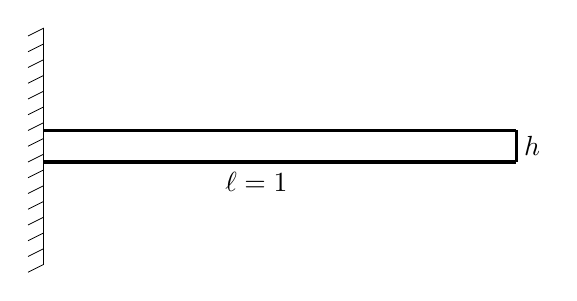
\begin{tikzpicture}
							\draw[line width = 0.4mm] (0,0.2) -- (6,0.2);
							\draw[line width = 0.4mm] (0,-0.2) -- (6,-0.2);
							\draw[line width = 0.4mm] (6,-0.2) -- (6,0.2);
							%\draw[line width = 0.4mm] (0,-0.2) -- (0,0.2);
							
							%\draw[line width = 0.1mm,->] (6,2) -- (7.4,2);
							%\draw[line width = 0.1mm,->] (6,2) -- (6,0.9);
							%\node at (6.7,1.8) {$e_1$};
							%\node at (5.8,1.4) {$e_2$};
							
							\node at (6.2,0) {$h$};
							\node at (2.7,-0.45) {$\ell = 1$};
							
							\draw[line width = 0.1mm] (0,-1.5) -- (0,1.5);
							\draw[line width = 0.1mm] (0,1.5) -- (-0.2,1.4);
							\draw[line width = 0.1mm] (0,1.3) -- (-0.2,1.2);
							\draw[line width = 0.1mm] (0,1.1) -- (-0.2,1);
							\draw[line width = 0.1mm] (0,0.9) -- (-0.2,0.8);
							\draw[line width = 0.1mm] (0,0.7) -- (-0.2,0.6);
							\draw[line width = 0.1mm] (0,0.5) -- (-0.2,0.4);
							\draw[line width = 0.1mm] (0,0.3) -- (-0.2,0.2);
							\draw[line width = 0.1mm] (0,0.1) -- (-0.2,0);
							
							\draw[line width = 0.1mm] (0,-0.1) -- (-0.2,-0.2);
							\draw[line width = 0.1mm] (0,-0.3) -- (-0.2,-0.4);
							\draw[line width = 0.1mm] (0,-0.5) -- (-0.2,-0.6);
							\draw[line width = 0.1mm] (0,-0.7) -- (-0.2,-0.8);
							\draw[line width = 0.1mm] (0,-0.9) -- (-0.2,-1);
							\draw[line width = 0.1mm] (0,-1.1) -- (-0.2,-1.2);
							\draw[line width = 0.1mm] (0,-1.3) -- (-0.2,-1.4);
							\draw[line width = 0.1mm] (0,-1.5) -- (-0.2,-1.6);
							
							%\node at (3.2,-0.3) {$\ell = 1$};
						
						\end{tikzpicture}
					\end{center}
					\subcaption{Two-Dimensional Cantilever Beam (Problem 2D)}
				\end{minipage}
			}
		}
	\end{figure}\label{fig:compare:1D+2D}

	\FloatBarrier

	In introduction of the Timoshenko beam model, the parameter $\alpha$ is introduced. The paramater is given here again for convenience:
	\begin{eqnarray*}
		\alpha = \frac{A\ell^2}{I}.
	\end{eqnarray*}

	The model is in a dimensionless form, therefore the length of the beam is $\ell = 1$. Since we assumed a square cross-section, the area of the cross-section can be calculated as $\displaystyle A = hb$. The area moment of inertia can also be calculated as $\displaystyle I = \frac{h^3b}{12}$. Substituting these values into the formula for $\alpha$ gives the following relationship between the height of the beam and the parameter $\alpha$: $\displaystyle \alpha = \frac{12}{h^2}$
	or equivalently,
	\begin{eqnarray}
		h & = & \sqrt{\frac{12}{\alpha}}. \label{eq:h-alpha-relationship}
	\end{eqnarray}
	Using this relationship, the height of the beam model can be set by considering the value of $\alpha$.

	\subsection*{Calculating the eigenvalues and eigenvectors}
	In the article \cite{VV02} a method for calculating the exact eigenvalues and eigenvectors of the Timoshenko beam is provided. For the two-dimensional beam, the eigenvalues and eigenvectors are calculated using the Finite Element Method, with setup in Section \ref{ssec:2D_Model:FEM}. The eigenvalue accuracy depends on the number of elements in the FEM. In the two-dimensional model, elements are selected to ensure the first 10 eigenvalues have at least 5 significant digits of accuracy.

	\subsection*{Comparing the mode shapes}
	Following \cite{LVV09}, the mode shapes of the two-models are compared. In the section that follows, we'll show that there are mode shapes that are shared between the models and mode shapes that are unique to the two-dimensional model. The authors of \cite{LVV09} refer to the eigenvalues of the Timoshenko beam model as beam-type eigenvalues and the other eigenvalues are referred to as non-beam type eigenvalues.

	Therefore a method is required to compare and match the eigenvalues of the two models. In \cite{LVV09}, the authors compare the mode shapes of the two models, to match up the eigenvalues. Eigenvalues relating to the mode shapes similar to the mode shapes of the Timoshenko beam, are called beam-type eigenvalues. The other eigenvalues are called non-beam type eigenvalues by the authors.


	\subsubsection*{Mode shapes relating to beam-type eigenvalues}

	Figure \ref{fig:beam1} shows examples of beam-type mode shapes for the displacement $w$.

	\begin{figure}[h!]
		\scalebox{.8}{
			\makebox[\textwidth][c]{
				\centering
				\begin{minipage}[b]{0.8\linewidth}
					\includegraphics[width=1\linewidth]{files/Chapter4/Beam1.jpg}
					\subcaption{2D Beam Type - $\lambda_6 = 21.911$}
					\label{fig:minipage2}
				\end{minipage}
				\begin{minipage}[b]{0.8\linewidth}
					\includegraphics[width=1\linewidth]{files/Chapter4/1DBeam2.png}
					\subcaption{Timoshenko - $\lambda_5 = 21.794$}
					\label{fig:minipage1}
				\end{minipage}
		}}
		\scalebox{.8}{
			\makebox[\textwidth][c]{
				\begin{minipage}[b]{0.8\linewidth}
					\includegraphics[width=1\linewidth]{files/Chapter4/Beam2.jpg}
					\subcaption{2D Beam Type - $\lambda_7 = 45.711$}
					\label{fig:minipage2}
				\end{minipage}
				\begin{minipage}[b]{0.8\linewidth}
					\includegraphics[width=1\linewidth]{files/Chapter4/1DBeam1.png}
					\subcaption{Timoshenko - $\lambda_6 = 45.390$}
					\label{fig:minipage1}
				\end{minipage}
				\caption{Modal shapes of the displacement $w$ for the beam-type 2D body and the Timoshenko beam with $\alpha = 4800$ ($h = 1/20$).}
				\label{fig:beam1}
			}
		}
	\end{figure}
	\FloatBarrier

	\subsubsection*{Mode shapes relating to non beam-type eigenvalues}
	Figure \ref{fig:beam2} shows examples of non beam-type mode shapes for the displacement $w$. These mode shapes are not present in the cantilever Timoshenko beam model and are not beam related. 
	\begin{figure}[h!]
		\scalebox{.8}{
			\makebox[\textwidth][c]{
				\centering
				\begin{minipage}[b]{0.8\linewidth}
					\includegraphics[width=1\linewidth]{files/Chapter4/NotBeam1.jpg}
					\subcaption{Non-Beam Type - $\lambda_4 = 7.7077$}
					\label{fig:minipage2}
				\end{minipage}
				\begin{minipage}[b]{0.8\linewidth}
					\includegraphics[width=1\linewidth]{files/Chapter4/NotBeam2.jpg}
					\subcaption{Non-Beam Type - $\lambda_8 = 69.344$}
					\label{fig:minipage1}
				\end{minipage}
				\caption{Modal shapes of the displacement $w$ for the non-beam type 2D body with $h = 1/20$.}
				\label{fig:beam2}
			}
		}
	\end{figure}
	\FloatBarrier

	\subsubsection*{Shape of the cross-section}
	The Timoshenko beam theory improve some one-dimensional beam theories such as the Euler-Bernoulli beam theory by also including the effect of shear. For Timoshenko beam theory it is assumed that the cross-sections need not remain perpendicular to the neutral axis of the beam. The cross-sections however remain a straight line.

	For the two-dimensional beam, the shape of the cross-section can deform into a S-shape. This is explained in \cite{LVV09} and a similar figure in \cite{LVV09} is given here. 

	\FloatBarrier
	\begin{figure}[h!]
		\centering
		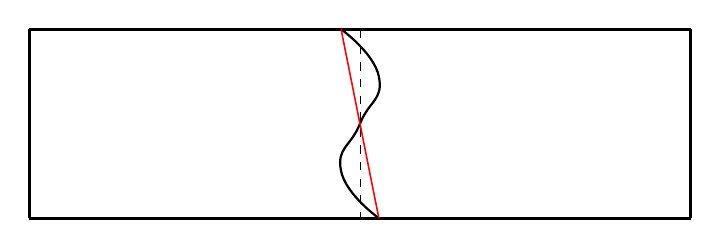
\begin{tikzpicture}[scale=1.2]
		
		\draw[line width = 0.4mm] (0,1) -- (7,1);
		\draw[line width = 0.4mm] (0,-1) -- (7,-1);
		\draw[line width = 0.4mm] (7,-1) -- (7,1);
		\draw[line width = 0.4mm] (0,-1) -- (0,1);
		
		
		\draw[line width = 0.1mm,dashed] (3.5,1) -- (3.5,-1);
		
		\draw[thick] plot [smooth,tension=0.9] coordinates{(3.3,1) (3.7,0.5) (3.5,0) (3.3,-0.5) (3.7,-1)};
		
		\draw[line width = 0.2mm,red] (3.3,1) -- (3.7,-1);
		
	\end{tikzpicture}
		\caption{S-shape deformation of the cross-section of the two-dimensional beam.}\label{fig:s}
	\end{figure}
	\FloatBarrier

	Note that figure \ref{fig:s} shows an exaggerated example of the deformation of a cross-section. The red line shows how the authors of \cite{LVV09} calculated the average rotation of a cross-section of the two-dimensional beam. This average rotation can be used to compare the rotation of the cross-section of the two-dimensional beam to the rotation of the cross-section of the Timoshenko beam given by $\phi$.

	\subsubsection*{Direct comparison of mode shapes}
	Figure \ref{fig:w} directly compares a mode shape of the Timoshenko beam to a mode shape of the two-dimensional beam. For the two-dimensional model, the center line of the displacement of the beam is shown. For the Timoshenko beam, the displacement $w$ is shown.

	\begin{figure}[ht!]
		\scalebox{.8}{
			\makebox[\textwidth]{
				\centering
				\centering
				\includegraphics[scale=0.4]{files/Chapter4/1Dv2D.png}
				\caption{Comparison of the displacement $w$ mode shape corresponding to $\lambda_{10}$ for the 2D beam and $\lambda_8$ for the Timoshenko beam with $\alpha = 4800$ ($h=1/20$)}
				\label{fig:w}}}
	\end{figure}
	\FloatBarrier

	Similarly, figure \ref{fig:phi} directly compares the angle of the cross-section of the Timoshenko beam and the two-dimensional beam. The average rotation of the cross-section of the two-dimensional beam's mode shape is calculated as shown in figure \ref{fig:s}.

	\FloatBarrier
	\begin{figure}[ht!]
		\scalebox{.8}{
			\makebox[\textwidth]{
				\centering
				\centering
				\includegraphics[scale=0.4]{files/Chapter4/1Dv2Dphi.png}
				\caption{Comparison of the angle $\phi$ (best fit for 2D Beam) mode shape corresponding to $\lambda_{10}$ for the 2D beam and $\lambda_8$ for the Timoshenko beam with $\alpha = 4800$ ($h=1/20$)}
				\label{fig:phi}}}
	\end{figure}
	\FloatBarrier

	These figures are examples that show how similar the mode shapes of the two models are. This specific example is for $\alpha = 4800$, which represents a typical beam. The authors of \cite{LVV09} obtained similar results for $\alpha=300$, which represents a short and thick beam.

	\textbf{Remark:} Note that the overall shape is important. This is because any multiple of a eigenvector is still an eigenvector. The mode shapes were specifically scaled to obtain figures \ref{fig:w} and \ref{fig:phi}.

	\subsection*{Comparing the eigenvalues}
	Using this method of comparing the mode shapes, the eigenvalues can now be matched up and compared. In the tables, Timo refers to the Timoshenko beam and 2D refers to the two-dimensional beam.

	\subsubsection*{Some results from \cite{LVV09}}
	The following table contains results from \cite{LVV09} verbatim to 3 significant digits, as well as the replicated results to 5 significant digits.

	\begin{table}[!ht]
		\centering
		\caption{Results from \cite{LVV09} and results obtained in this dissertation. $0^*$ indicates a 0 as a result of rounding. $\alpha = 1200$.}
		\begin{tabular}{|c|c|c||c|c|c|}
			\hline
			\multicolumn{3}{|c||}{Results from \cite{LVV09}} & \multicolumn{3}{c|}{Dissertation} \\ \hline \hline
			~ & 2D & Timo & ~ & 2D & Timo  \\ \hline
			1 & 0.0317 & 0.0316 & 1 & 0.031713 & 0.031639  \\ 
			2 & 1.14 & 1.14  & 2 & 1.1413 & 1.1365  \\ 
			3 & 7.72 & - & 3 & 7.7161 & - \\ 
			4 & 7.92 & 7.86 &  4 & 7.918 & 7.8617    \\ 
			5 & 26.2 & 25.9 & 5 & 26.148 & 25.869   \\ 
			6 & 60.8 & 59.9 & 6 & 60.816 & 59.946  \\ 
			7 & 69.3 & - & 7 & 69.344 & -  \\ 
			8 & 115 & 113 &  8 & 115.28 & 113.23   \\ 
			9 & 192 & 188 &  9 & 191.57 & 187.55   \\ 
			10 & 192 & - & 10 & 192.03 & -  \\ 
			11 & 291 & 284 & 11 & 290.76 & 283.81   \\ \hline
		\end{tabular}\label{Results_LVV09}
	\end{table}


	\begin{comment}
	\begin{table}[!ht]
		\centering
		\caption{Results from \cite{LVV09} and results obtained in this dissertation. $0^*$ indicates a 0 as a result of rounding. $\alpha = 1200$.}
		\begin{tabular}{|c|c|c|c||c|c|c|c|}
			\hline
			\multicolumn{4}{|c||}{Results from \cite{LVV09}} & \multicolumn{4}{c|}{Dissertation} \\ \hline \hline
			~ & 2D & Timo & RE & ~ & 2D & Timo & RE  \\ \hline
			1 & 0.0317 & 0.0316 & 0.00315 & 1 & 0.031713 & 0.031639 & 0.0023407  \\ 
			2 & 1.14 & 1.14 & $0^*$ & 2 & 1.1413 & 1.1365 &  0.0042050 \\ 
			3 & 7.72 & - & ~ & 3 & 7.7161 & - &   \\ 
			4 & 7.92 & 7.86 & 0.00758 & 4 & 7.918 & 7.8617 & 0.0071116    \\ 
			5 & 26.2 & 25.9 & 0.0115 & 5 & 26.148 & 25.869 & 0.010669  \\ 
			6 & 60.8 & 59.9 & 0.0148 & 6 & 60.816 & 59.946 & 0.014303  \\ 
			7 & 69.3 & - & ~ & 7 & 69.344 & - &    \\ 
			8 & 115 & 113 & 0.0174 & 8 & 115.28 & 113.23 &  0.017787  \\ 
			9 & 192 & 188 & 0.0208 & 9 & 191.57 & 187.55 &  0.020999  \\ 
			10 & 192 & - &  & 10 & 192.03 & - &   \\ 
			11 & 291 & 284 & 0.0241 & 11 & 290.76 & 283.81 &  0.023899  \\ \hline
		\end{tabular}\label{Results_LVV09}
	\end{table}
	\end{comment}


	This table shows that the results obtained in this dissertation are very similar to the results obtained in \cite{LVV09}. This is for a specific case where $\alpha = 1200$.

	In the following table, the eigenvalues for different values of $\alpha$ are compared.

	\begin{table}[h!]
		\scalebox{.8}{
		\makebox[\textwidth]{
		\caption{Eigenvalues of a Timoshenko cantilever beam vs the eigenvalues of a cantilever two-dimensional elastic body. *RE is the relative error.}
		\begin{tabular}{|cccc||cccc||cccc||cccc|}
			\hline
			\multicolumn{16}{|c|}{Comparison of Eigenvalues} \\
			\hline\hline
			\multicolumn{4}{|c||}{ $h = 1/5$ or $\alpha = 300$}       & \multicolumn{4}{c||}{$h =1/10$ or $\alpha = 1200$}      & \multicolumn{4}{c||}{$h = 1/20$ or $\alpha = 4800$}      & \multicolumn{4}{c|}{$h = 1/30$ or $\alpha = 10800$} \\
			\hline
			{i} & {2D} & {j} & {Timo} & {i} & {2D} & {j} & {Timo} & {i} & {2D} & {j} & {Timo} & {i} & {2D} & {j} & {Timo} \\
			\hline
			{1}&0.12151&1&0.12092&1&0.031713&1&0.031639&1&0.008013&1&0.008004&1&0.003568&1&0.003565\\
			{2}&3.5460&2&3.5071&2&1.1413&2     & 1.1365 & 2     & 0.30756 & 2     & 0.30705 & 2     & 0.13869 & 2     & 0.13855 \\
			\cellcolor{lightgray}{3} & \cellcolor{lightgray}{7.7311} &       & {-} & \cellcolor{lightgray}{3}     & \cellcolor{lightgray}{7.7161} &       & {-} & 3     & 2.3273 & 3     & 2.3213 & 3     & 1.0698 & 3     & 1.0683 \\
			{4} & 20.225 & 3     & 19.869 & 4     & 7.9180 & 3     & 7.8617 & \cellcolor{lightgray}{4}     & \cellcolor{lightgray}{7.7077} &       & {-} & 4     & 4.0140 & 4     & 4.0058 \\
			{5} & 56.109 & 4     & 54.766 & 5     & 26.148 & 4     & 25.869 & 5     & 8.5086 & 4     & 8.4762 & \cellcolor{lightgray}{5}     & \cellcolor{lightgray}{7.7047} &       & {-} \\
			\cellcolor{lightgray}{6} & \cellcolor{lightgray}{69.164} &       & {-} & 6     & 60.816 & 5     & 59.946 & 6     & 21.911 & 5     & 21.794 & 6     & 10.655 & 5     & 10.625 \\
			{7} & 114.03 & 5     & 110.75 & \cellcolor{lightgray}{7}     & \cellcolor{lightgray}{69.344} &       & {-} & 7     & 45.711 & 6     & 45.390 & 7     & 22.975 & 6     & 22.890 \\
			{8} & {189.17} &  6     & {186.50} & 8     & 115.28 & 6     & 113.23 & \cellcolor{lightgray}{8}     & \cellcolor{lightgray}{69.344} &       & {-} & 8     & 43.113 & 7     & 42.909 \\
			\cellcolor{lightgray}{9} & \cellcolor{lightgray}{192.61} &      &  & {9}     & {191.57} &   7  & {187.55} & 9     & 82.887 & 7     & 82.154 & \cellcolor{lightgray}{9}     & \cellcolor{lightgray}{69.331} &       & {-} \\
			{10} & 285.85 & 7     & 277.64 & \cellcolor{lightgray}{10}    & \cellcolor{lightgray}{192.03} &      & {-} & 10    & 136.03 & 8     & 134.58 & 10    & 73.230 & 8     & 72.803 \\
			{11} & 328.40 & 8     & 330.29 & 11    & 290.76 & 8     & 283.81 & \cellcolor{lightgray}{11}    & \cellcolor{lightgray}{192.48} &       & {-} & 11    & 115.41 & 9     & 114.61 \\
			\cellcolor{lightgray}{12} & \cellcolor{lightgray}{357.08} &       & {-} & \cellcolor{lightgray}{12}    & \cellcolor{lightgray}{374.45} &       & {-} & 12    & 207.29 & 9     & 204.69 & 12    & 171.61 & 10    & 170.20 \\
			{13} & 397.33 & 9     & 394.02 & 13    & 413.20 & 9     & 402.27 & 13    & 298.38 & 10    & 294.10 & \cellcolor{lightgray}{13}    & \cellcolor{lightgray}{192.52} &       & {-} \\
			{14} & 442.00   & 10    & 439.52 & 14    & 558.67 & 10    & 542.65 & \cellcolor{lightgray}{14}    & \cellcolor{lightgray}{376.83} &       & {-} & 14    & 243.56 & 11    & 241.26 \\
			\cellcolor{lightgray}{15} & \cellcolor{lightgray}{533.71} &       & {-} & \cellcolor{lightgray}{15}    & \cellcolor{lightgray}{614.11} &       & {-} & 15    & 410.63 & 11    & 404.01 & 15    & 332.83 & 12    & 329.28 \\
			{16} & 538.97 & 11    & 541.55 & 16    & 726.26 & 11    & 704.15 & 16    & 545.03 & 12    & 535.32 & \cellcolor{lightgray}{16}    & \cellcolor{lightgray}{377.16} &       & {-} \\
			\cellcolor{lightgray}{17} & \cellcolor{lightgray}{596.06} &       & {-} & \cellcolor{lightgray}{17}    & \cellcolor{lightgray}{906.28} &       & {-} & \cellcolor{lightgray}{17}    & \cellcolor{lightgray}{621.95} &       & {-} & 17    & 440.77 & 13    & 435.51 \\
			{18} & 602.77 & 12    & 596.09 & 18    & 913.69 & 12    & 884.92 & 18    & 702.30 & 13    & 688.64 & 18    & 568.51 & 14    & 561.04 \\
			\cellcolor{lightgray}{19} & \cellcolor{lightgray}{657.87} &       & {-} & 19    & 1113.7 & 13    & 1080.1 & 19    & 882.95 & 14    & 864.40 & \cellcolor{lightgray}{19}    & \cellcolor{lightgray}{623.05} &       & {-} \\
			{20} & 717.37 & 13    & 731.74 & \cellcolor{lightgray}{20}    & \cellcolor{lightgray}{1218.0}  &       & {-} & \cellcolor{lightgray}{20}    & \cellcolor{lightgray}{927.18} &       & {-} & 20    & 717.04 & 15    & 706.74 \\
			\hline
			\multicolumn{2}{|c}{Max RE:} & \multicolumn{2}{c||}{3.1718\%} & \multicolumn{2}{c}{Max RE:} & \multicolumn{2}{c||}{3.1486\%} & \multicolumn{2}{c}{Max RE:} & \multicolumn{2}{c||}{2.1018\%} & \multicolumn{2}{c}{Max RE:} & \multicolumn{2}{c|}{1.4361\%} \\
			\hline
		\end{tabular}%
		\label{tab:Timo}%
	}
	}
	\end{table}%
	\FloatBarrier

	This table shows that the eigenvalues of the Timoshenko model and the two-dimensional model compare very well. The non-beam type eigenvalues are highlighted in grey. For a short thick beam ($\alpha = 300$), the maximum relative error for the first 20 two-dimensional eigenvalues is just over $3\%$, while for a long thin beam ($\alpha = 10800$), the maximum relative error is just over $1\%$. This shows that as the beam becomes longer and thinner, the Timoshenko beam is better approximation of the two-dimensional beam. But overall the Timoshenko beam compares very well.

	This table also shows that as the beam gets more narrow, there are less non-beam type eigenvalues within the first few eigenvalues.This would also indicate that the Timoshenko beam would be a better approximation of the two-dimensional beam as the beam gets more narrow since the two-dimensional model behaves `more like a beam'.

\section{Validity of a model for a cantilever two-dimensional beam} \label{sec:validity-of-a-2d-beam}
In this section, we compare the two-dimensional cantilever beam with a three-dimensional cantilever beam.

Figure \ref{fig:2Dv3D} shows the two beams, Problem 2D and Problem 3D side-by-side.

\FloatBarrier
\begin{figure}[h!]
	\scalebox{.8}{
		\makebox[\textwidth][c]{
			\caption{Side-by-side comparison of the beams.}
			\label{fig:2Dv3D}
			\centering
			\begin{minipage}[b]{0.7\linewidth}
				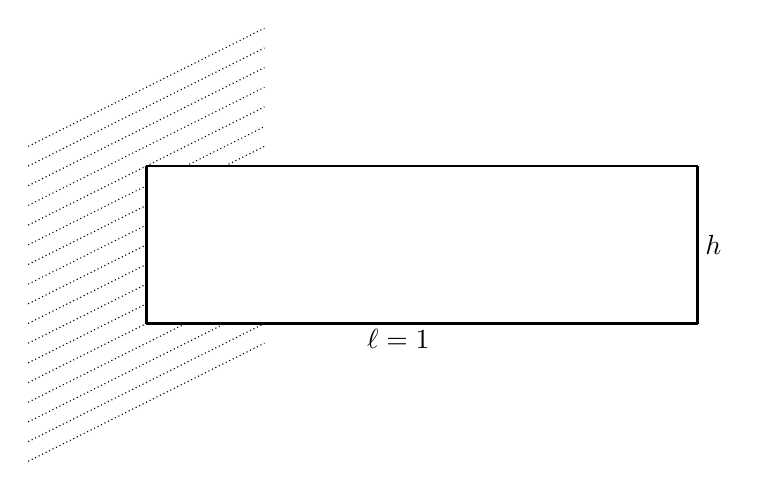
\begin{tikzpicture}
					\draw[line width = 0.3mm] (0,1) -- (7,1);
					\draw[line width = 0.3mm] (0,-1) -- (7,-1);
					\draw[line width = 0.3mm] (7,-1) -- (7,1);
					\draw[line width = 0.3mm] (0,-1) -- (0,1);
					
					
					\draw[scale=0.5, domain=-3:3, smooth, variable=\x,densely dotted] plot ({\x}, {0.5*\x+4});
					\draw[scale=0.5, domain=-3:3, smooth, variable=\x,densely dotted] plot ({\x}, {0.5*\x+3.5});
					\draw[scale=0.5, domain=-3:3, smooth, variable=\x,densely dotted] plot ({\x}, {0.5*\x+3});
					\draw[scale=0.5, domain=-3:3, smooth, variable=\x,densely dotted] plot ({\x}, {0.5*\x+2.5});
					\draw[scale=0.5, domain=-3:3, smooth, variable=\x,densely dotted] plot ({\x}, {0.5*\x+2});
					
					\draw[scale=0.5, domain=-3:0, smooth, variable=\x,densely dotted] plot ({\x}, {0.5*\x+1.5});
					\draw[scale=0.5, domain=-3:0, smooth, variable=\x,densely dotted] plot ({\x}, {0.5*\x+1});
					
					
					\draw[scale=0.5, domain=1:3, smooth, variable=\x,densely dotted] plot ({\x}, {0.5*\x+1.5});
					\draw[scale=0.5, domain=2:3, smooth, variable=\x,densely dotted] plot ({\x}, {0.5*\x+1});
					
					\draw[scale=0.5, domain=-3:0, smooth, variable=\x,densely dotted] plot ({\x}, {0.5*\x+0.5});
					\draw[scale=0.5, domain=-3:0, smooth, variable=\x,densely dotted] plot ({\x}, {0.5*\x});
					\draw[scale=0.5, domain=-3:0, smooth, variable=\x,densely dotted] plot ({\x}, {0.5*\x-0.5});
					\draw[scale=0.5, domain=-3:0, smooth, variable=\x,densely dotted] plot ({\x}, {0.5*\x-1});
					\draw[scale=0.5, domain=-3:0, smooth, variable=\x,densely dotted] plot ({\x}, {0.5*\x-1.5});
					\draw[scale=0.5, domain=-3:0, smooth, variable=\x,densely dotted] plot ({\x}, {0.5*\x-2});
					\draw[scale=0.5, domain=-3:1, smooth, variable=\x,densely dotted] plot ({\x}, {0.5*\x-2.5});
					\draw[scale=0.5, domain=-3:2, smooth, variable=\x,densely dotted] plot ({\x}, {0.5*\x-3});
					\draw[scale=0.5, domain=-3:3, smooth, variable=\x,densely dotted] plot ({\x}, {0.5*\x-3.5});
					\draw[scale=0.5, domain=-3:3, smooth, variable=\x,densely dotted] plot ({\x}, {0.5*\x-4});
					
					\node at (7.2,0) {$h$};
					\node at (3.2,-1.2) {$\ell = 1$};
				\end{tikzpicture}
				\subcaption{Two-Dimensional Elastic Body}
			\end{minipage}
			\begin{minipage}[b]{0.7\linewidth}
				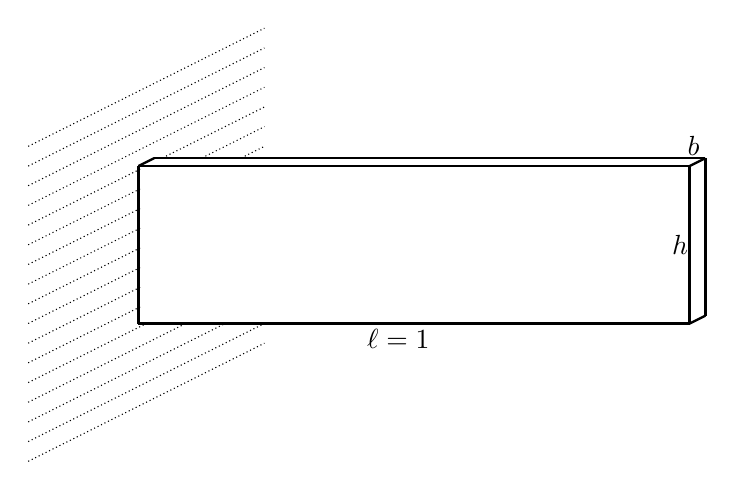
\begin{tikzpicture}
					\draw[line width = 0.3mm] (-0.1,1) -- (6.9,1);
					\draw[line width = 0.3mm] (-0.1,-1) -- (6.9,-1);
					\draw[line width = 0.3mm] (6.9,-1) -- (6.9,1);
					\draw[line width = 0.3mm] (-0.1,-1) -- (-0.1,1);
					
					\draw[line width = 0.3mm] (0.1,1.1) -- (7.1,1.1);
					\draw[line width = 0.3mm] (7.1,-0.9) -- (7.1,1.1);
					
					\draw[line width = 0.3mm] (-0.1,1) -- (0.1,1.1);
					\draw[line width = 0.3mm] (6.9,1) -- (7.1,1.1);
					\draw[line width = 0.3mm] (6.9,-1) -- (7.1,-0.9);
					
					
					
					\draw[scale=0.5, domain=-3:3, smooth, variable=\x,densely dotted] plot ({\x}, {0.5*\x+4});
					\draw[scale=0.5, domain=-3:3, smooth, variable=\x,densely dotted] plot ({\x}, {0.5*\x+3.5});
					\draw[scale=0.5, domain=-3:3, smooth, variable=\x,densely dotted] plot ({\x}, {0.5*\x+3});
					\draw[scale=0.5, domain=-3:3, smooth, variable=\x,densely dotted] plot ({\x}, {0.5*\x+2.5});
					
					\draw[scale=0.5, domain=-3:-0.1, smooth, variable=\x,densely dotted] plot ({\x}, {0.5*\x+2});
					\draw[scale=0.5, domain=-3:-0.1, smooth, variable=\x,densely dotted] plot ({\x}, {0.5*\x+1.5});
					\draw[scale=0.5, domain=-3:-0.1, smooth, variable=\x,densely dotted] plot ({\x}, {0.5*\x+1});
					
					\draw[scale=0.5, domain=0.5:3, smooth, variable=\x,densely dotted] plot ({\x}, {0.5*\x+2});
					\draw[scale=0.5, domain=1.5:3, smooth, variable=\x,densely dotted] plot ({\x}, {0.5*\x+1.5});
					\draw[scale=0.5, domain=2.5:3, smooth, variable=\x,densely dotted] plot ({\x}, {0.5*\x+1});
					
					\draw[scale=0.5, domain=-3:-0.1, smooth, variable=\x,densely dotted] plot ({\x}, {0.5*\x+0.5});
					\draw[scale=0.5, domain=-3:-0.1, smooth, variable=\x,densely dotted] plot ({\x}, {0.5*\x});
					\draw[scale=0.5, domain=-3:-0.1, smooth, variable=\x,densely dotted] plot ({\x}, {0.5*\x-0.5});
					\draw[scale=0.5, domain=-3:-0.1, smooth, variable=\x,densely dotted] plot ({\x}, {0.5*\x-1});
					\draw[scale=0.5, domain=-3:-0.1, smooth, variable=\x,densely dotted] plot ({\x}, {0.5*\x-1.5});
					\draw[scale=0.5, domain=-3:0, smooth, variable=\x,densely dotted] plot ({\x}, {0.5*\x-2});
					\draw[scale=0.5, domain=-3:1, smooth, variable=\x,densely dotted] plot ({\x}, {0.5*\x-2.5});
					\draw[scale=0.5, domain=-3:2, smooth, variable=\x,densely dotted] plot ({\x}, {0.5*\x-3});
					\draw[scale=0.5, domain=-3:3, smooth, variable=\x,densely dotted] plot ({\x}, {0.5*\x-3.5});
					\draw[scale=0.5, domain=-3:3, smooth, variable=\x,densely dotted] plot ({\x}, {0.5*\x-4});
					
					\node at (6.95,1.25) {$b$};
					\node at (6.78,0) {$h$};
					\node at (3.2,-1.2) {$\ell = 1$};
					

				\end{tikzpicture}
				\subcaption{Three-Dimensional Elastic Body}
				
			\end{minipage}
		}
	}
\end{figure}
\FloatBarrier

\subsection*{Calculating the eigenvalues and mode shapes}
 The accuracy of the eigenvalues depends on the number of elements employed in the finite element method. For the two-dimensional model, accuracy reaches at least five significant digits for the first 10 eigenvalues, while the three-dimensional model achieves at least four significant digits for its first 10 eigenvalues.

\subsection*{Comparing the mode shapes}
Following the same method as \cite{LVV09}, the mode shapes of the two models are compared. As seen in \cite{LVV09} and Section \ref{sec:validity-of-a-cantilever-timoshenko-beam}, the eigenvalues of the Timoshenko beam model (beam-type eigenvalues) are all present in the two-dimensional model. However not all the eigenvalues of the two-dimensional model are present in the Timoshenko beam model. These are called non-beam type eigenvalues. 

The same is observed for the three-dimensional model, as there are eigenvalues that are present in the three-dimensional model that are not present in the two-dimensional model. Therefore it is required to match the eigenvalues of the two models by comparing the mode shapes.

\subsubsection*{Mode shapes relating to beam type eigenvalues.}
Figure \ref{fig:beam-2dv3d} show some examples of beam type mode shapes for the displacement $u$.

\begin{figure}[h!]
	\scalebox{.8}{
		\makebox[\textwidth][c]{
			\centering
			\begin{minipage}[b]{0.8\linewidth}
				\includegraphics[width=1\linewidth]{files/Chapter6/3D12.png}
				\subcaption{3D Beam Type - $\lambda_{12} = 2.3293$}
				\label{fig:minipage2}
			\end{minipage}
			\begin{minipage}[b]{0.8\linewidth}
				\includegraphics[width=1\linewidth]{files/Chapter6/2D3.png}
				\subcaption{2D Beam Type - $\lambda_3 = 2.3273$}
				\label{fig:minipage1}
			\end{minipage}
	}}
	\scalebox{.8}{
		\makebox[\textwidth][c]{
			\centering
			\begin{minipage}[b]{0.8\linewidth}
				\includegraphics[width=1\linewidth]{files/Chapter6/3D22.png}
				\subcaption{3D Beam Type - $\lambda_{24} = 21.929$}
				\label{fig:minipage2}
			\end{minipage}
			\begin{minipage}[b]{0.8\linewidth}
				\includegraphics[width=1\linewidth]{files/Chapter6/2D6.png}
				\subcaption{2D Beam Type - $\lambda_6 = 21.911$}
				\label{fig:minipage1}
			\end{minipage}
			\caption{Mode shapes of the displacement $u$ with $h=1/20$.}
			\label{fig:beam-2dv3d}
	}}
\end{figure}
\FloatBarrier

\subsubsection*{Mode shapes relating to non-beam type eigenvalues that are present in the two-dimensional model.}
Figure \ref{fig:nonbeam-2dv3d} show examples of mode shapes relating to non-beam type eigenvalues for the displacement $u$.

\FloatBarrier
\begin{figure}[h!]
	\scalebox{.8}{
		\makebox[\textwidth][c]{
			\centering
			\begin{minipage}[b]{0.8\linewidth}
				\includegraphics[width=1\linewidth]{files/Chapter6/3D33.png}
				\subcaption{3D Non-Beam Type - $\lambda_{33} = 69.374$}
				\label{fig:minipage2}
			\end{minipage}
			\begin{minipage}[b]{0.8\linewidth}
				\includegraphics[width=1\linewidth]{files/Chapter6/2D8.png}
				\subcaption{2D Non-Beam Type - $\lambda_8 = 69.344$}
				\label{fig:minipage1}
			\end{minipage}
			\caption{Mode shapes of the displacement $u$ with $h=1/20$.}
			\label{fig:nonbeam-2dv3d}
	}}
\end{figure}
\FloatBarrier

\subsubsection*{Mode shapes relating to non-beam type eigenvalues that are not present in the two-dimensional model.}
Figure \ref{fig:nonbeam-2dv3d} show examples of mode shapes relating to non-beam type eigenvalues for the displacement $u$ which are not present in the two-dimensional model. These mode shapes only appear in the three-dimensional beam.
\FloatBarrier
\begin{figure}[h!]
	\scalebox{.8}{
		\makebox[\textwidth][c]{
			\centering
			\begin{minipage}[b]{0.8\linewidth}
				\includegraphics[width=1\linewidth]{files/Chapter6/3DNonBeam10.png}
				\subcaption{Non-2D Type - $\lambda_{10}$}
				\label{fig:minipage2}
			\end{minipage}
			\begin{minipage}[b]{0.8\linewidth}
				\includegraphics[width=1\linewidth]{files/Chapter6/3DNonBeam11.png}
				\subcaption{Non-2D Type - $\lambda_{11}$}
				\label{fig:minipage11}
			\end{minipage}
			\caption{Mode shapes of the displacement $u$ with $h=1/20$.}
			
	}}
\end{figure}
\FloatBarrier

\subsection*{Comparing the eigenvalues}
For a realistic comparison of the models, it's crucial to carefully select parameters $h$ and $b$, representing the beam's height and width, respectively, noting that the two-dimensional model lacks the width parameter $b$.

Values for $h$ span a range from short, thick beams ($h = 1/5$) to long, slender beams ($h = 1/20$), capturing two realistic scenarios. Regarding $b$, it's considered in two scenarios: when $b \leq h$ and when $b > h$, with $b$ expressed as a multiple of $h$. This distinction influences the results.

Results will cover all shared eigenvalues between the models, highlighting non-beam type eigenvalues in grey. Non-beam type eigenvalues unique to either model are excluded, but eigenvalue numbering will proceed as if they were included.

\subsubsection*{Case $b \leq h$:}
Table \ref{tab:2v3_1} below compares the eigenvalues of the models for a beam with a small length to height ratio of $h=1/5$ with decreasing values of $b$. 

\begin{table}[htbp]
	\scalebox{.8}{
	\makebox[\textwidth]{
		\caption{Comparsion of Eigenvalues with $h = 1/5$, with decreasing $b$ and $b < h$.}
		\begin{tabular}{|cc|cc|cc|cc||cc|}
			\hline
			\multicolumn{10}{|c|}{Eigenvalues} \\
			\hline
			\hline
			i     & {b = h} & i     & {b = 1/2 h} & i     & {b = 1/4 h} & i     & {b = 1/8 h} & j     & 2D \\
			\hline
			{2} & 0.12307 & {2} & 0.12234 & {2} & 0.12198 & {3} & 0.12178 & 1     & 0.12151 \\
			{3} & 3.5773 & {5} & 3.5630 & {6} & 3.5558 & {8} & 3.5519 & 2     & 3.5460 \\
			\rowcolor{lightgray}{5} & 7.7799 & {6} & 7.7596 & {8} & 7.7471 & {11} & 7.7401 & 3     & 7.7311 \\
			{8} & 20.334 & {9} & 20.283 & {11} & 20.26 & {14} & 20.247 & 4     & 20.225 \\
			{10} & 56.247 & {12} & 56.173 & {15} & 56.156 & {22} & 56.142 & 5     & 56.109 \\
			\rowcolor{lightgray}{11} & 69.197 & {14} & 69.319 & {17} & 69.281 & {24} & 69.238 & 6     & 69.164 \\
			{14} & 114.03 & {16} & 114.01 & {20} & 114.05 & {29} & 114.06 & 7     & 114.03 \\
			\rowcolor{lightgray}{17} & 187.01 & {19} & 189.14 & {25} & 189.37 & {36} & 189.34 & 8     & 189.17 \\
			{18} & 192.21 & {20} & 192.41 & {26} & 192.58 & {37} & 192.63 & 9     & 192.61 \\
			{21} & 284.76 & {23} & 285.43 & {31} & 285.74 & {42} & 285.84 & 10    & 285.85 \\
			{23} & 327.57 & {26} & 328.24 & {35} & 328.37 & {46} & 328.40 & 11    & 328.40 \\
			\rowcolor{lightgray}{25} & 347.77 & {28} & 356.44 & {36} & 357.30 & {50} & 357.33 & 12    & 357.08 \\
			{27} & 393.69 & {30} & 396.84 & {38} & 397.28 & {53} & 397.37 & 13    & 397.33 \\
			{30} & 434.46 & {34} & 441.05 & {41} & 441.81 & {57} & 441.99 & 14    & 442.00 \\
			\rowcolor{lightgray}{31} & 523.65 & {36} & 534.04 & {43} & 534.17 & {63} & 534.03 & 15    & 533.71 \\
			{34} & 550.51 & {37} & 537.82 & {44} & 538.86 & {64} & 539.06 & 16    & 538.97 \\
			\rowcolor{lightgray}{37} & 590.86 & {41} & 587.43 & {48} & 594.17 & {65} & 595.58 & 17    & 596.06 \\
			{39} & 590.86 & {42} & 600.52 & {49} & 602.25 & {67} & 602.69 & 18    & 602.77 \\
			\rowcolor{lightgray}{42} & 646.21 & {44} & 657.22 & {50} & 658.04 & {71} & 658.06 & 19    & 657.87 \\
			{44} & 711.07 & {46} & 714.62 & {53} & 717.10 & {73} & 717.51 & 20    & 717.37 \\
			\hline
			\hline
			\multicolumn{2}{|c|}{Max RE: \  2.6069\%} &\multicolumn{2}{c|}{Max RE: \ 1.4469\%}  & \multicolumn{2}{c|}{Max RE: \  0.38192\%}  & \multicolumn{2}{c||}{Max RE: \ 0.22301\%}& \multicolumn{2}{c|}{-} \\
			\hline
		\end{tabular}%
		\label{tab:2v3_1}%
	}}
\end{table}%
\FloatBarrier
\label{sym:RE}

% Table generated by Excel2LaTeX from sheet 'Sheet2'
\begin{table}[htbp]
	\centering
	\caption{Maximum relative error for beam type and non-beam type eigenvalues for $h = 1/5$.}
	\begin{tabular}{|c|cccc|}
		\hline
		\multicolumn{5}{|c|}{Maximum Relative Error} \\
		\hline
		\hline
		& {b = h} & {b = 1/2h} & {b = 1/4h} & {b = 1/8h} \\
		\hline
		Beam Type & 2.1420 \% & 0.6804 \% & 0.38192 \% & 0.22301 \% \\
		Non-Beam Type & 2.6069 \% & 1.4469 \% & 0.31546 \% & 0.11680 \% \\
		\hline
	\end{tabular}%
	\label{tab:2Dv3D_1_breakup}%
\end{table}%

Table \ref{tab:2v3_1} below compares the eigenvalues of the models for a beam with a larger length to height ratio of $h=1/20$ with decreasing values of $b$. 

\begin{table}[ht]
	\scalebox{.8}{
	\makebox[\textwidth]{
	\caption{Comparsion of Eigenvalues with $h = 1/20$, with decreasing $b$ and $b < h$.}
	\begin{tabular}{|cc|cc|cc|cc||cc|}
		\hline
		\multicolumn{10}{|c|}{Eigenvalues} \\
		\hline
		\hline
		i     & {b = h} & i     & {b = 1/2 h} & i     & {b = 1/4 h} & i     & {b = 1/8 h} & j     & 2D \\
		\hline
		{2} & 0.008043 & {2} & 0.008029 & {2} & 0.008023 & {3} & 0.00802 & {1} & {0.008013} \\
		{3} & 0.3087 & {4} & 0.30816 & {5} & 0.30794 & {7} & 0.30785 & {2} & {0.30757} \\
		{5} & 2.3357 & {8} & 2.3316 & {9} & 2.3300  & {12} & 2.3293 & {3} & {2.3273} \\
		\rowcolor{lightgray}{8} & 7.7217 & {10} & 7.7156 & {13} & 7.7124 & {16} & 7.7111 & {4} & {7.7077} \\
		{10} & 8.5387 & {11} & 8.5238 & {14} & 8.5182 & {18} & 8.516 & {5} & {8.5086} \\
		{11} & 21.986 & {14} & 21.948 & {18} & 21.934 & {24} & 21.929 & {6} & {21.911} \\
		{14} & 45.863 & {18} & 45.781 & {21} & 45.756 & {30} & 45.746 & {7} & {45.712} \\
		\rowcolor{lightgray}{17} & 69.444 & {19} & 69.408 & {25} & 69.385 & {33} & 69.374 & {8} & {69.344} \\
		{18} & 83.149 & {22} & 82.999 & {27} & 82.960 & {36} & 82.944 & {9} & {82.887} \\
		{21} & 136.44 & {25} & 136.19 & {31} & 136.14 & {42} & 136.12 & {10} & {136.03} \\
		\rowcolor{lightgray}{23} & 192.62 & {27} & 192.62 & {35} & 192.58 & {47} & 192.56 & {11} & {192.48} \\
		{25} & 207.87 & {29} & 207.5 & {36} & 207.43 & {48} & 207.41 & {12} & {207.29} \\
		{27} & 299.14 & {33} & 298.63 & {41} & 298.56 & {55} & 298.53 & {13} & {298.38} \\
		\rowcolor{lightgray}{30} & 376.68 & {35} & 377.01 & {44} & 377.01 & {58} & 376.98 & {14} & {376.83} \\
		{31} & 411.58 & {37} & 410.89 & {46} & 410.83 & {61} & 410.81 & {15} & {410.63} \\
		{34} & 546.15 & {40} & 545.27 & {50} & 545.24 & {66} & 545.23 & {16} & {545.03} \\
		\rowcolor{lightgray}{37} & 620.77 & {42} & 622.02 & {53} & 622.19 & {69} & 622.18 & {17} & {621.95} \\
		{39} & 703.55 & {44} & 702.49 & {54} & 702.29 & {71} & 702.53 & {18} & {702.31} \\
		{42} & 884.27 & {47} & 883.02 & {59} & 883.14 & {82} & 883.19 & {19} & {882.96} \\
		\rowcolor{lightgray}{44} & 923.68 & {49} & 926.88 & {60} & 927.43 & {86} & 927.50 & {20} & {927.18} \\
		\hline
		\hline
		\multicolumn{2}{|c|}{Max RE: \  0.37701\%} &\multicolumn{2}{c|}{Max RE: \ 0.19893\%}  & \multicolumn{2}{c|}{Max RE: \  0.12393\%}  & \multicolumn{2}{c||}{Max RE: \ 0.092843\%}& \multicolumn{2}{c|}{-} \\
		\hline
	\end{tabular}%
	\label{tab:2v3_2}%
}}
\end{table}%
\FloatBarrier

\begin{table}[htbp]
	\centering
	\caption{Maximum relative error for beam type and non-beam type eigenvalues for $h = 1/20$}
	\begin{tabular}{|c|cccc|}
		\hline
		\multicolumn{5}{|c|}{Maximum Relative Error} \\
		\hline
		\hline
		& {b = h} & {b = 1/2h} & {b = 1/4h} & {b = 1/8h} \\
		\hline
		Beam Type & 0.37701 \% & 0.19893 \% & 0.12393 \% & 0.092843 \% \\
		Non-Beam Type & 0.37682 \% & 0.10218 \% & 0.061213 \% & 0.043601 \% \\
		\hline
	\end{tabular}%
	\label{tab:2v3_2_split}%
\end{table}%
\FloatBarrier


Tables \ref{tab:2v3_1} and \ref{tab:2v3_2} show that the first 20 eigenvalues of the two-dimensional model closely match those of the three-dimensional beam for $b \leq h$. As width $b$ decreases, the two-dimensional model approximates the three-dimensional model more accurately. The comparison is notably better for the slender beam with $h = 1/20$ than for the thick beam with $h = 1/5$, though both comparisons are strong.

The tables also indicate an increase in non-beam type eigenvalues in the three-dimensional model as both $b$ and $h$ decrease.

Tables \ref{tab:2Dv3D_1_breakup} and \ref{tab:2v3_2_split} show the maximum relative error for beam type and non-beam type eigenvalues, confirming the close comparison of beam type eigenvalues.


\subsubsection*{Case $b > h$:}
First, the case is considered where $h = 1/5$.

\FloatBarrier
\begin{table}[htbp]
	\scalebox{.8}{
	\makebox[\textwidth]{
		\caption{Comparsion of Eigenvalues with $h = 1/5$, with increasing $b$ and $b > h$}
		\begin{tabular}{|cc|cc|cc||cc|}
			\hline
			\multicolumn{8}{|c|}{Eigenvalues} \\
			\hline
			\hline
			i     & {b = 2h} & i     & {b = 4h} & i     & {b = 8h} & j     & 2D \\
			\hline
			{1} & 0.12474 					& {1} & 0.12766 & {1} & 0.13036 & 1     & 0.12151 \\
			{4} & 3.6088 					& {4} & 3.6297 & {5} & 3.7766 & 2     & 3.5460 \\
			\rowcolor{lightgray}{6} & 7.8091 & {5} & 7.8389 & {9} & 8.9239 & 3     & 7.7311 \\
			{8} & 20.466 					& {9} & 20.959 & {15} & 21.031 & 4     & 20.255 \\
			{11} & 56.309					& {18} & 58.149 & {30} & 60.862 & 5     & 56.109 \\
			\hline
			\hline
			\multicolumn{2}{|c|}{Max RE: \  2.6603\%} &\multicolumn{2}{c|}{Max RE: \ 5.0571\%}  & \multicolumn{2}{c|}{Max RE: \  15.428\%} & \multicolumn{2}{c|}{-} \\
			\hline
		\end{tabular}%
		\label{tab:b>h}%
	}}
\end{table}
\FloatBarrier

\FloatBarrier
\begin{table}[htbp]
	\centering
	\caption{Maximum relative error for beam type and non-beam type eigenvalues for $h = 1/5$}
	\begin{tabular}{|c|ccc|}
		\hline
		\multicolumn{4}{|c|}{Maximum Relative Error} \\
		\hline
		\hline
		& {b = 2h} & {b = 4h} & {b = 8h} \\
		\hline
		Beam Type & 2.6603 \% & 5.0571 \% & 8.4712 \% \\
		Non-Beam Type & 1.0096 \% & 1.3948 \% & 15.428 \% \\
		\hline
	\end{tabular}%
	\label{tab:b>h-split}%
\end{table}%
\FloatBarrier

In Table \ref{tab:b>h}, the height of the beam is set to $h=1/20$, which was the best case when $b<h$.

\FloatBarrier
\begin{table}[htbp]
	\scalebox{.8}{
	\makebox[\textwidth]{
		\caption{Comparsion of Eigenvalues with $h = 1/20$, with increasing $b$ and $b > h$}
		\begin{tabular}{|cc|cc|cc||cc|}
			\hline
			\multicolumn{8}{|c|}{Eigenvalues} \\
			\hline
			\hline
			i     & {b = 2h} & i     & {b = 4h} & i     & {b = 8h} & j     & 2D \\
			\hline
			{2} & 0.008076 & {1} & 0.008162 & {1} & 0.008324 & 1     & 0.008013 \\
			{3} & 0.30995 & {3} & 0.31298 & {3} & 0.31738 & 2     & 0.30757 \\
			{5} & 2.3462 & {5} & 2.3737 & {6} & 2.4116 & 3     & 2.3273 \\
			\rowcolor{lightgray}{8} & 7.7312 & {8} & 7.7471 & {9} & 7.7711 & 4     & 7.7077 \\
			{10} & 8.5841 & {9} & 8.7082 & {10} & 8.7929 & 5     & 8.5086 \\
			{11} & 22.124 & {12} & 22.491 & {14} & 23.222 & 6     & 21.911 \\
			{14} & 46.195 & {14} & 47.003 & {18} & 47.921 & 7     & 45.712 \\
			\rowcolor{lightgray}{17} & 69.454 & {17} & 69.281 & {22} & 72.307 & 8     & 69.344 \\
			{18} & 83.822 & {18} & 85.218 & {24} & 80.607 & 9     & 82.887 \\
			{21} & 137.43 & {21} & 138.58 & {32} & 140.97 & 10    & 136.03 \\
			\hline
			\hline
			\multicolumn{2}{|c|}{Max RE: \  1.1289\%} &\multicolumn{2}{c|}{Max RE: \ 2.8261\%}  & \multicolumn{2}{c|}{Max RE: \  5.9821\%} & \multicolumn{2}{c|}{-} \\
			\hline
		\end{tabular}%
		\label{tab:b>h_20}%
	}}
\end{table}
\FloatBarrier

\FloatBarrier
\begin{table}[htbp]
	\centering
	\caption{Maximum relative error for beam type and non-beam type eigenvalues for $h = 1/20$}
	\begin{tabular}{|c|ccc|}
		\hline
		\multicolumn{4}{|c|}{Maximum Relative Error} \\
		\hline
		\hline
		& {b = 2h} & {b = 4h} & {b = 8h} \\
		\hline
		Beam Type & 1.1289 \% & 2.8261 \% & 5.9821 \% \\
		Non-Beam Type & 0.30521 \% & 0.51096 \% & 4.2734 \% \\
		\hline
	\end{tabular}%
	\label{tab:b>h-split_20}%
\end{table}%
\FloatBarrier

Tables \ref{tab:b>h} and \ref{tab:b>h_20} indicate that the two-dimensional model's accuracy declines when $b$ significantly exceeds $h$, a trend also observed for beam type eigenvalues in Tables \ref{tab:b>h-split} and \ref{tab:b>h-split_20}. Particularly for $h=1/5$, obtaining reliable eigenvalues numerically was challenging.

These results comprehensively assess the two-dimensional cantilever beam model against the three-dimensional counterpart, demonstrating good agreement across a broad spectrum of beam shapes, especially in scenarios representing realistic cases.

The key takeaway is the critical role of beam shape: the two-dimensional model performs excellently when $b \leq h$, particularly for slender beams, but less so for short, thick beams. The model's accuracy rapidly deteriorates as $b$ surpasses $h$, affecting both slender and short, thick beams, with the latter posing challenges in numerical eigenvalue calculation.

For practical applications, a beam model's suitability is questionable when $b > h$, suggesting alternative approaches like plate models for more accurate representation. The next section explores the Reissner-Mindlin plate model's validity using a similar analysis.

\section{Conclusion} \label{sec:conclusion}
In this article, we assessed the validity of both a cantilever Timoshenko beam model and a two-dimensional cantilever beam model by comparing their eigenvalues and mode shapes. Initially, we evaluated the Timoshenko beam model's validity by comparison with the two-dimensional model, as per the article \cite{LVV09}. Subsequently, the validity of the two-dimensional model was examined through comparison with a three-dimensional model.

The models were given in a dimensionless variational form, and we demonstrated how the two-dimensional model could be derived from the three-dimensional model as a specific case of plane stress.

While we did not delve into the well-posedness of the models in detail, we cited necessary references. The principle of modal analysis was illustrated with a general example, proving essential for comparing the two models. This comparison's application is evident in the numerical results presented in this article.

Applying the Finite Element Method to both models, we developed a numerical formula for solving the eigenvalue problems. A computer program was then used to extract the eigenvalues and eigenvectors for each model.

Firstly, the results of \cite{LVV09} is confirmed, showing that the Timsohenko canitlever beam model comapres very well to the two-dimensional model. The models compare very well if the beams are long and slender, and good for short and thick beams. Extending this to the three-dimensional model, we found that the two-dimensional model aligns well with the three-dimensional model for various beam shapes. Again we found that the shape of the beam is pivotal to the comparison's accuracy. The two-dimensional model shows the best correlation with thin and long three-dimensional beams and less so with short and thick beams. Notably, the two-dimensional model does not align well when the beam's width $b$ exceeds its height $h$, suggesting that a plate model may be more appropriate in such cases and can be explored in future work.

\bibliographystyle{elsarticle-harv}
\bibliography{references}

\end{document}